\documentclass[11pt]{amsart}

\usepackage[T1]{fontenc}
\usepackage{lmodern}
\usepackage{amsmath,amssymb,amsthm}
\usepackage[a4paper,margin=1.15in]{geometry}
\usepackage{microtype}

\usepackage{xcolor}
\definecolor{ink}{HTML}{2E3A59}
\definecolor{bellA}{HTML}{3B74B8}
\definecolor{bellB}{HTML}{E07B39}
\definecolor{soft}{HTML}{8A8F9C}
\definecolor{famA}{HTML}{3B74B8}
\definecolor{famB}{HTML}{E07B39}
\definecolor{famC}{HTML}{2A9D8F}
\definecolor{famD}{HTML}{B5446E}
\definecolor{famE}{HTML}{6C5B7B}

\usepackage{tikz}
\usetikzlibrary{calc}
\usepackage{pgfplots}
\pgfplotsset{compat=1.18}
\usepackage{booktabs}
\usepackage{enumitem}
\setlist{itemsep=0.1em, topsep=0.3em}
\usepackage[font=small,labelfont=sc,labelsep=period,figurename=Figure]{caption}
\usepackage[colorlinks,linkcolor=black,citecolor=black,urlcolor=bellA]{hyperref}

% Theorem heads: a provenance marker set by \mnew or \mgpt just before the
% environment is printed right after the upright period that ends the head.
\newcommand{\thmmarker}{}
\newcommand{\mnew}{\gdef\thmmarker{\textsuperscript{$\star$}}}
\newcommand{\mgpt}{\gdef\thmmarker{\textsuperscript{$\dagger$}}}
\newcommand{\markedhead}[3]{\thmname{#1}\thmnumber{ #2}%
  \thmnote{ {\normalfont(#3)}}{\normalfont.\thmmarker}\gdef\thmmarker{}}
\newcommand{\thmskip}{0.5\baselineskip plus 0.2\baselineskip minus 0.2\baselineskip}
\newtheoremstyle{tplain}{\thmskip}{\thmskip}{\itshape}{}{\bfseries}%
  {}{5pt plus 1pt minus 1pt}{\markedhead{#1}{#2}{#3}}
\newtheoremstyle{tdefinition}{\thmskip}{\thmskip}{\normalfont}{}{\bfseries}%
  {}{5pt plus 1pt minus 1pt}{\markedhead{#1}{#2}{#3}}
\newtheoremstyle{tremark}{\thmskip}{\thmskip}{\normalfont}{}{\itshape}%
  {}{5pt plus 1pt minus 1pt}{\markedhead{#1}{#2}{#3}}
\theoremstyle{tplain}
\newtheorem{theorem}{Theorem}[section]
\newtheorem{lemma}[theorem]{Lemma}
\newtheorem{corollary}[theorem]{Corollary}
\newtheorem{proposition}[theorem]{Proposition}
\theoremstyle{tdefinition}
\newtheorem{definition}[theorem]{Definition}
\newtheorem{example}[theorem]{Example}
\theoremstyle{tremark}
\newtheorem{remark}[theorem]{Remark}

\newcommand{\lmin}{\lambda_{\min}}
\newcommand{\tr}{\operatorname{tr}}
\newcommand{\NN}{\mathbb N}
\newcommand{\ZZ}{\mathbb Z}
\newcommand{\new}{\textsuperscript{$\star$}}
\newcommand{\gpt}{\textsuperscript{$\dagger$}}

\urlstyle{tt}
\newcommand{\doi}[1]{\href{https://doi.org/#1}{\nolinkurl{doi:#1}}}
\newcommand{\arxiv}[1]{\href{https://arxiv.org/abs/#1}{\nolinkurl{arXiv:#1}}}
\newcommand{\Diag}{\operatorname{Diag}}
\newcommand{\SDP}{\operatorname{SDP}}

\title{Tools for proving that graphs are not graceful}
\author{Boon Suan Ho}
\date{Version 2, 18 October 2026}

\begin{document}

\begin{abstract}
A graph with $m$ edges is graceful if its vertices can be labeled with
distinct integers in $[0,m]$ whose edge differences are exactly $1,\dots,m$.
Graceful labelings have been constructed for sixty years, but there are few
general methods for showing that a graph is \emph{not} graceful. We start
from a single generating-function identity that restates gracefulness, and
derive three tools from it: residues at roots of unity, extending the
classical parity condition; positivity on the unit circle, whose semidefinite form amounts exactly to
the Goemans--Williamson max-cut relaxation tested against the
minimum of the Dirichlet kernel; and the label interval itself, which forces the labels of a dense subgraph
to have a large span. The consequences include new families of
ungraceful graphs: every edge-transitive graph that contains $K_6$, the Paley graphs $P(q)$ with $q\ge37$, the Kneser
graphs $K(n,k)$ with $n\ge5.61\,k$, almost every $d$-regular graph with
$d\ge84$, and the polarity graphs $\mathrm{ER}_q$ with $q\ge23$, which contain no
$4$-cycle. For the semidefinite form of positivity we also
determine exactly what it can prove, and we show that a planar refinement is strictly stronger: it excludes the Kneser graph $K(11,2)$ with any seven edges deleted.
\end{abstract}

\maketitle

\begin{center}
\fbox{\parbox{0.9\textwidth}{\small\textbf{About this article.} The text of this article was written by
Claude Opus~5.5, an AI model made by Anthropic, at the direction of Boon Suan
Ho, who chose the questions and steered the work. Version~2 incorporates
corrections and new results from a revision by GPT-6 Pro (OpenAI), and some of
its passages are adapted from that revision. Results marked~\new\ were found
by Claude, and results marked~\gpt\ by GPT-6 Pro. The author has not checked
every proof in detail. Section~\ref{sec:provenance} gives the
details.}}
\end{center}

% ----------------------------------------------------------------
\section{Introduction}\label{sec:intro}

A graph $G$ with $m$ edges is \emph{graceful} if there is an injective map
$f\colon V(G)\to\{0,1,\ldots,m\}$ such that the edge differences
$|f(u)-f(v)|$, $uv\in E(G)$, are exactly $1,2,\ldots,m$. These labelings were
introduced by Rosa~\cite{rosa65,rosa} under the name $\beta$-valuations, and
named by Golomb~\cite{golomb}. Gallian's dynamic survey~\cite{gallian} lists
thousands of papers, almost all of which \emph{construct} graceful labelings.
Figure~\ref{fig:k4} shows a small example, and a connection that runs through
this paper: on a complete subgraph, a graceful labeling is a \emph{Golomb
ruler}, a set of marks whose pairwise distances are all different.

\begin{figure}[ht]
\centering
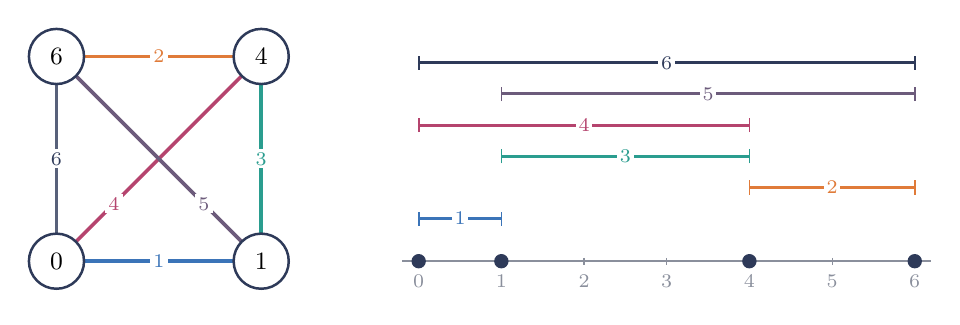
\begin{tikzpicture}[
    vtx/.style={circle, draw=ink, fill=white, line width=0.9pt, minimum size=7mm, inner sep=0pt, font=\small},
    dif/.style={fill=white, inner sep=1.2pt, font=\scriptsize}]
  % the graph K_4
  \begin{scope}
    \coordinate (v0) at (0,0); \coordinate (v1) at (2.6,0);
    \coordinate (v4) at (2.6,2.6); \coordinate (v6) at (0,2.6);
    \draw[famA, line width=1.3pt] (v0) -- node[dif, text=famA] {1} (v1);
    \draw[famB, line width=1.3pt] (v6) -- node[dif, text=famB] {2} (v4);
    \draw[famC, line width=1.3pt] (v1) -- node[dif, text=famC] {3} (v4);
    \draw[famD, line width=1.3pt] (v0) -- node[dif, text=famD, pos=0.28] {4} (v4);
    \draw[famE, line width=1.3pt] (v1) -- node[dif, text=famE, pos=0.28] {5} (v6);
    \draw[ink!80, line width=1.3pt] (v0) -- node[dif, text=ink] {6} (v6);
    \node[vtx] at (v0) {0}; \node[vtx] at (v1) {1};
    \node[vtx] at (v4) {4}; \node[vtx] at (v6) {6};
  \end{scope}
  % the ruler
  \begin{scope}[xshift=4.6cm, x=1.05cm, y=0.36cm]
    \draw[soft, line width=0.6pt] (-0.2,0) -- (6.2,0);
    \foreach \x in {0,...,6} \draw[soft] (\x,0.12) -- (\x,-0.12);
    \foreach \x in {0,...,6} \node[soft, font=\scriptsize, below] at (\x,-0.15) {\x};
    \foreach \x in {0,1,4,6} \fill[ink] (\x,0) circle (2.6pt);
    \foreach \a/\b/\d/\c in {0/1/1/famA, 4/6/2/famB, 1/4/3/famC, 0/4/4/famD, 1/6/5/famE, 0/6/6/ink} {
      \draw[\c, line width=1.1pt] (\a,1.1*\d+0.4) -- (\b,1.1*\d+0.4);
      \draw[\c, line width=0.6pt] (\a,1.1*\d+0.15) -- (\a,1.1*\d+0.65);
      \draw[\c, line width=0.6pt] (\b,1.1*\d+0.15) -- (\b,1.1*\d+0.65);
      \node[\c, font=\scriptsize, fill=white, inner sep=1pt] at ({(\a+\b)/2},1.1*\d+0.4) {\d};
    }
  \end{scope}
\end{tikzpicture}
\caption{A graceful labeling of $K_4$: the six edges have differences
$1,\dots,6$. Since $K_4$ is complete, this says that the marks $0,1,4,6$ measure
every distance from $1$ to $6$ exactly once. Such a ruler is a \emph{perfect
Golomb ruler}, and none exists with five or more marks.}
\label{fig:k4}
\end{figure}

\begin{table}[t]
\centering\footnotesize
\setlength{\tabcolsep}{3.5pt}
\begin{tabular}{@{}lll@{}}
\toprule
\textbf{family} & \textbf{not graceful when} & \textbf{source}\\
\midrule
\multicolumn{3}{@{}l}{\emph{Tool I: parity and residues}}\\
graphs with all degrees even & $m\equiv1,2\pmod 4$ & Bos\'ak~\cite{rosa65}; Cor.~\ref{cor:rosa}\\
friendship graphs $K_3^{(t)}$ & $t\equiv2,3\pmod4$ & Bos\'ak~\cite{rosa65}; Ex.~\ref{ex:windmills}\\
windmills $K_5^{(t)}$ & $t$ odd, or $t=2,4$ & \cite{rosa65,bkt,kt77,mo}; Rem.~\ref{rem:windmills}\\
decompositions into an odd number of $K_5$'s & always & Cor.~\ref{cor:decomp}\\
graphs split into two or three $K_4$'s & any overlap & \cite{bkt}; Prop.~\ref{prop:iterated}\\
$K_s\vee\overline K_{2t}$ & $s\equiv8,10\pmod{16}$ & Cor.~\ref{cor:splitparity}\gpt\\
$K_{8k+6}\vee\overline K_{2t}$ & $k+t$ odd & Cor.~\ref{cor:gauss}\gpt\\
\midrule
\multicolumn{3}{@{}l}{\emph{Tool II: positivity, with clique and density certificates}}\\
complete graphs $K_n$ & $n\ge5$ & Golomb~\cite{golomb}; Cor.~\ref{cor:cliques}\\
windmills $K_n^{(t)}$; unions $tK_n$ & $n\ge6$ & \cite{koh,kotzig}; Cor.~\ref{cor:cliques}\\
barbells $B_n$ & $n\ge6$ & Cor.~\ref{cor:cliques}\new\\
$K_n\square P_r$, $K_n\square C_r$ & $n\ge13$ (all $r$) & Li~\cite{knuth-err}; Cor.~\ref{cor:cliques}\\
graphs with $m\ge0.4108\,n^2$ edges & always & \cite{rr,leech}; Cor.~\ref{cor:dense}\\
complete multipartite $K_{a_1,\dots,a_r}$ & $\sum a_i^2\le\frac{\kappa}{1+\kappa}n^2+1$ & Cor.~\ref{cor:dense}\\
graphs decomposing into $K_n$'s & $n\ge6$ & \cite{bkt}; Thm.~\ref{thm:cliquedec}\\
mixed or fractional decompositions into $K_{\ge6}$'s & always & Thm.~\ref{thm:cliquedec}\new\\
edge-transitive graphs containing $K_6$ & always & Cor.~\ref{cor:decomp}\new\\
$t$ copies of $K_n$ sharing a $K_r$ & $n\ge2.4r+6$, all $t$ & Cor.~\ref{cor:bnrt}\new\\
line graphs of linear hypergraphs $H$ & $\delta(H)\ge6$ & Cor.~\ref{cor:drg}\new\\
\quad triangular graphs $T(n)$ & $n\ge7$ & Cor.~\ref{cor:drg}\new\\
\quad rook's graphs $K_a\square K_b$ & $a+b\ge12$; $K_2\square K_9$, $K_3\square K_8$ & Cor.~\ref{cor:drg}\new\\
gen.\ quadrangles $\mathrm{GQ}(s,t)$; nets of order $n$ & $s\ge5$;\ $n\ge6$ & Cor.~\ref{cor:drg}\new\\
Hamming graphs $H(d,q)$ & $q\ge6$, every $d$ & Cor.~\ref{cor:drg}\new\\
Johnson graphs $J(n,k)$, $k\le n/2$ & $n\ge k+5$ & Cor.~\ref{cor:drg}\new\\
Grassmann graphs $J_q(n,k)$ & all but $K_3,K_4$ & Cor.~\ref{cor:drg}\new\gpt\\
$q$-Kneser graphs $K_q(n,k)$, $k\ge2$ & all but $K_2(4,2)$ (open) & Cor.~\ref{cor:drg}\gpt\\
\midrule
\multicolumn{3}{@{}l}{\emph{Tool II: positivity, through eigenvalues}}\\
Kneser graphs $K(n,k)$ & $n\ge5.61\,k$ & Cor.~\ref{cor:drg}\new\\
Paley graphs $P(q)$ & $q\ge37$ & Cor.~\ref{cor:paley}\new\\
graphs with $\lmin\ge-2$ & avg.\ degree $\ge9.21$ & Cor.~\ref{cor:spec2}\new\\
non-bipartite Ramanujan graphs & degree $\ge84$ & Cor.~\ref{cor:spec2}\new\\
random $d$-regular graphs & $d\ge84$, a.a.s. & Cor.~\ref{cor:random}\new\\
polarity graphs $\mathrm{ER}_q$ (no $C_4$) & $q\ge23$ & Cor.~\ref{cor:spec2}\new\gpt\\
\midrule
\multicolumn{3}{@{}l}{\emph{Tool II: the planar refinement}}\\
$K(11,2)$ minus $\le7$ edges; blowups, unions & always & Cor.~\ref{cor:kg}\gpt\\
\midrule
\multicolumn{3}{@{}l}{\emph{Tool III: the interval}}\\
$K_r$ plus $\lfloor r^2/4\rfloor$ leaves at one vertex & $r\ge46$ & Cor.~\ref{cor:leaves}\gpt\\
$t$ edge-disjoint $K_{20}$'s plus $\le59t+4$ edges & always & Cor.~\ref{cor:packing}\gpt\\
\bottomrule
\end{tabular}
\caption{Ungraceful families obtained in this paper. In the last column, a
citation gives the first proof we know of, and a reference to a numbered
result gives the proof here. The markers \new\ and \gpt\ indicate results that
we believe are new (a row with both was found partly by each); see
Section~\ref{sec:provenance}. Here $\kappa\approx0.2172$ is Leech's constant
(Lemma~\ref{lem:dirichlet}); notation is explained at the end of
Section~\ref{sec:intro}.}
\label{tab:families}
\end{table}

For a single graph the two directions are not symmetric. A labeling is a
certificate of gracefulness that anyone can check, but in general there is no
short certificate of the opposite, and an exhaustive search must rule out
every injection of $n$ vertices into $m+1$ labels. For a whole family the
difficulty can lie on either side: the conjecture of Ringel and Kotzig that
every tree is graceful~\cite{gallian} has resisted both proof and
counterexample for sixty years. For the negative direction, the classical
tools are Bos\'ak's parity condition, published by
Rosa~\cite{rosa65,rosa}, and Golomb's related partition
condition~\cite{golomb}, together with case-by-case arguments and computer
searches. We derive three tools, each applicable to every graph, from a
single identity, and apply them to the families in Table~\ref{tab:families}.

All three start from the same observation. If the edge differences of a
labeling are exactly $1,\dots,m$, then the generating function of the
differences is known in advance:
\[
  \sum_{uv\in E}\bigl(z^{f(u)-f(v)}+z^{f(v)-f(u)}\bigr)=\sum_{0<|k|\le m}z^k .
\]
The left side depends on the graph and the labeling; the right side does not.
The identity sees only differences along edges, so it does not record that
the labels are \emph{distinct integers in $[0,m]$}: on a path with three
edges, the labels $0,1,3,0$ satisfy it too. Tool~I evaluates it at roots of
unity and Tool~II on the unit circle. Tools~I and~III
also use part of this missing information (the capacities of residue
classes, and the bounded span of the labels); Tool~II needs only the identity
itself, combined with positivity:

\begin{enumerate}[label=\textbf{\Roman*.}]
\item \textbf{Parity and residues} (Section~\ref{sec:parity}). At $z=-1$, and
  more generally at roots of unity, the identity counts edges by the residues
  of their endpoints' labels; the extra information is that each residue class
  of $[0,m]$ holds only so many labels. This gives the classical conditions of
  Bos\'ak and Golomb, an iterated form that is strictly stronger
  (Proposition~\ref{prop:iterated}), and integer equations for the residues of
  labels.
\item \textbf{Positivity on the unit circle} (Section~\ref{sec:positivity}).
  At $z=e^{it}$ the right side is $D_m(t)-1$, where $D_m$ is the Dirichlet
  kernel, whose minimum is below $-\kappa(2m+1)$. On the left, replacing each label $x$ by the point $e^{itx}$ turns the
  sum into a quadratic form in these points, and positive semidefinite matrices bound this form from below; the bound
  is strong for graphs close to unions of cliques and weak for graphs with a
  large cut. The
  resulting criterion
  (Theorem~\ref{thm:P}) has a spectral form, a combinatorial form (\emph{a
  graph whose edges decompose, even fractionally, into cliques of order at
  least $6$ is not graceful}), and an exact description as a max-cut
  relaxation.
\item \textbf{The interval} (Section~\ref{sec:interval}). Labels are distinct
  integers in $[0,m]$, so a dense subgraph, which needs many distinct
  differences, forces a long label span. It excludes graphs that neither iterated parity nor positivity excludes
(Proposition~\ref{prop:missed}).
\end{enumerate}

For positivity we determine exactly what its semidefinite form can prove
(Proposition~\ref{prop:maxcut}), and show that a planar refinement proves strictly more
(Section~\ref{sec:planar}); for parity we give graphs it does not exclude (Section~\ref{sec:cannot}),
and we show that the interval excludes graphs that iterated parity and
positivity both miss (Proposition~\ref{prop:missed}); open cases that no tool
reaches are collected in Section~\ref{sec:open}. Table~\ref{tab:families} lists the
families covered, grouped by tool. A few examples: every graph whose edges
split into cliques with at least six vertices is not graceful (for cliques
of one order this is, in the language of difference sets, a theorem of
Bermond, Kotzig and Turgeon~\cite{bkt}), and neither is
any edge-transitive graph that contains $K_6$; nor almost any $d$-regular graph
with $d\ge84$; nor the polarity graphs $\mathrm{ER}_q$ for $q\ge23$, which
contain no $4$-cycle. Section~\ref{sec:provenance} records the history
and the origin of each result, and Section~\ref{sec:open} collects open
problems, among them the Beutner--Harborth conjecture on complete
multipartite graphs.

\emph{How to read this paper.} We assume only basic linear algebra (eigenvalues,
positive semidefinite matrices), a little elementary number theory, and
standard graph theory. After Section~\ref{sec:identity}, the three tools can be read independently
(except Proposition~\ref{prop:missed}, which compares them). Each tool comes with a guiding example: cycles and
$K_9$ for parity, complete graphs for positivity, and a clique with pendant
leaves for the interval. Section~\ref{sec:dictionary} is background and can be
skipped.

\emph{Notation.} Graphs are finite and simple; $G$ has $n$ vertices and $m$
edges, and we assume $m\ge1$ (a graph with no edges is graceful exactly when
it has at most one vertex). A labeling is a map $f\colon V(G)\to\{0,\dots,m\}$, and
$d_{uv}=|f(u)-f(v)|$ is the difference on the edge $uv$. We write $K_n$, $C_n$
and $P_n$ for the complete graph, the cycle and the path on $n$ vertices,
$K_{a_1,\dots,a_r}$ for the complete multipartite graph with parts of sizes
$a_1,\dots,a_r$, and $\overline K_N$ for $N$ isolated vertices. $G\vee H$ is
the join (every vertex of $G$ joined to every vertex of $H$), $G\square H$ the
Cartesian product, $tK_n$ the disjoint union of $t$ copies of $K_n$, and
$K_n^{(t)}$ the windmill of $t$ copies of $K_n$ sharing one vertex.
$A$ is the adjacency matrix, $J$ the all-ones matrix, $\lmin$ the smallest
eigenvalue of~$A$, and $M\succeq0$ means that $M$ is positive semidefinite.
The Dirichlet kernel $D_m$, the trial frequency $t^*$, the number
$\beta_m=1-\min_tD_m(t)$, and the constant $\kappa=0.2172\ldots$ (Leech's
constant, minus the minimum of $\sin x/x$) are defined in
Lemma~\ref{lem:dirichlet}. Other
families of graphs are defined where they first appear.


% ----------------------------------------------------------------
\section{The master identity}\label{sec:identity}

Let $f$ be a graceful
labeling of $G$, and for each edge $e=uv$ let $d_e=|f(u)-f(v)|$. Since
$\{d_e\}=\{1,\ldots,m\}$, we have, as Laurent polynomials in $z$ (each edge
contributes its difference with both signs),
\begin{equation}\label{eq:master}
  \sum_{uv\in E}\bigl(z^{f(u)-f(v)}+z^{f(v)-f(u)}\bigr)
  \;=\;\sum_{0<|k|\le m}z^k .
\end{equation}
The identity is elementary: it restates the definition as a generating
function. For a complete graph it reads $A(z)A(z^{-1})=n+\sum_{0<|k|\le m}z^k$
with $A(z)=\sum_vz^{f(v)}$, the familiar equation for Golomb rulers and, in
cyclic form, for difference sets~\cite{bjl}; R\'edei and R\'enyi~\cite{rr} and
Leech~\cite{leech} used it on the unit circle, and Clark, Curtis, Gnang and
Hogben~\cite{ccgh} relate graceful labelings to matrices of roots of unity.
For the labeling of $K_4$ in Figure~\ref{fig:k4} both sides are
$z^{-6}+\dots+z^{-1}+z+\dots+z^6$. On the unit circle the right-hand side is $D_m(t)-1$, where $D_m$ is the
Dirichlet kernel.

\begin{lemma}[Dirichlet kernel]\label{lem:dirichlet}
For $t\notin2\pi\ZZ$,
\[
  D_m(t):=1+2\sum_{k=1}^m\cos kt=\frac{\sin\bigl((m+\frac12)t\bigr)}{\sin(t/2)}.
\]
Let $\alpha\approx4.4934$ be the root of $\tan\alpha=\alpha$ in
$(\pi,\frac32\pi)$, and put
\[
  \kappa=-\min_{x>0}\frac{\sin x}{x}=-\frac{\sin\alpha}{\alpha}=0.21723362821\ldots,\qquad
  \beta_m=1-\min_tD_m(t).
\]
Then at the \emph{trial frequency} $t^*=2\alpha/(2m+1)$, which lies in the
first interval where $D_m<0$, we have
$D_m(t^*)<-\kappa(2m+1)$, so $\beta_m>1+\kappa(2m+1)$.
\end{lemma}

\begin{proof}
Multiply by $\sin(t/2)$ and use
$2\sin(t/2)\cos kt=\sin((k+\frac12)t)-\sin((k-\frac12)t)$; the sum telescopes.
At $t=2\alpha/(2m+1)$ the numerator is $\sin\alpha<0$, and the denominator is
$\sin\bigl(\alpha/(2m+1)\bigr)<\alpha/(2m+1)$, so the value is below
$-\kappa(2m+1)$. That $\alpha$ gives the global minimum of $\sin x/x$: the
function is nonnegative on $[0,\pi]$, has its unique minimum on $[\pi,2\pi]$
at $\alpha$, and for $x\ge2\pi$ its absolute value is at most
$1/(2\pi)<2/(3\pi)$, while its value at $\frac32\pi$ is $-2/(3\pi)$.
\end{proof}

Where does $\kappa$ come from? Put $x=(m+\frac12)t$. For large $m$ and small
$t$, $\sin(t/2)\approx t/2$, so $D_m(t)\approx(2m+1)\,\sin x/x$: the kernel is
a stretched copy of $\sin x/x$, whose deepest point is $-\kappa$ at
$x=\alpha$. In words, as $m\to\infty$ the $m$ cosines $\cos kt$ can be made to average
about $-\kappa\approx-0.217$, and no lower. For finite $m$ the minimum lies below $-\kappa(2m+1)$; $\beta_m$ records its
exact value, and $\kappa$ gives
convenient uniform bounds (Lemma~\ref{lem:betabound} bounds $\beta_m$ from
above). Every bound in Tool~II is stated in terms of~$\kappa$.

R\'edei and R\'enyi~\cite{rr} used the point $3\pi/(2m+1)$, where the
numerator is $-1$; it gives the constant $2/(3\pi)\approx0.2122$ in place of
$\kappa$. Leech~\cite{leech} used the minimum of $\sin x/x$, which gives
$\kappa$. Neither point is exactly the minimum of $D_m$ for finite $m$: the
critical points satisfy $\tan x=N\tan(x/N)$, where $N=2m+1$ and $x=Nt/2$, and
the first one tends to $\alpha$ as $m\to\infty$. Figure~\ref{fig:kernel} shows the first dip.

\begin{figure}[ht]
\centering
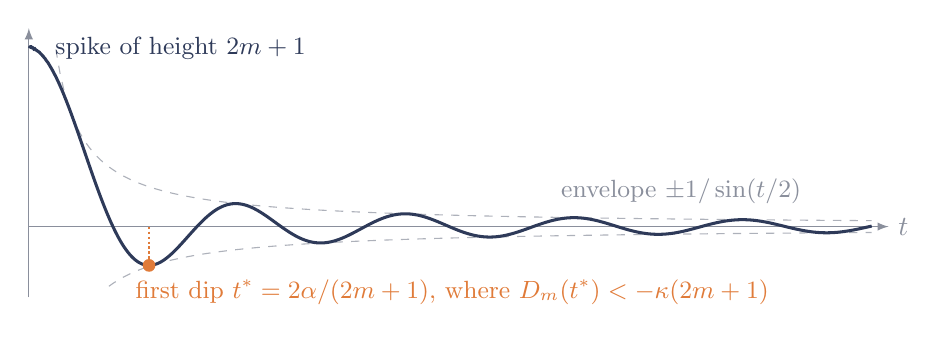
\begin{tikzpicture}
\begin{axis}[
    width=12.5cm, height=5.0cm,
    axis lines=middle, axis line style={soft, -latex},
    xmin=0, xmax=1.02, ymin=-25, ymax=70,
    xtick=\empty, ytick=\empty,
    xlabel={$t$}, xlabel style={at={(ticklabel* cs:1)}, anchor=west, soft},
    clip=false,
  ]
  \addplot[soft!70, dashed, domain=0.032:1, samples=200] {1/sin(deg(x/2))};
  \addplot[soft!70, dashed, domain=0.095:1, samples=200] {-1/sin(deg(x/2))};
  \addplot[ink, line width=1.1pt, domain=0.0004:1, samples=900] {sin(deg(31.5*x))/sin(deg(x/2))};
  \draw[bellB, densely dotted, line width=0.8pt] (axis cs:0.1426,0) -- (axis cs:0.1426,-13.70);
  \fill[bellB] (axis cs:0.1426,-13.70) circle (2.3pt);
  \node[bellB, anchor=north west, font=\small] at (axis cs:0.115,-15.2)
     {first dip $t^*=2\alpha/(2m+1)$, where $D_m(t^*)<-\kappa(2m+1)$};
  \node[ink, anchor=west, font=\small] at (axis cs:0.02,63) {spike of height $2m+1$};
  \node[soft, anchor=south west, font=\small] at (axis cs:0.62,4.6) {envelope $\pm 1/\sin(t/2)$};
\end{axis}
\end{tikzpicture}
\caption{The Dirichlet kernel $D_m(t)$ for $m=31$. Every positivity argument in
Section~\ref{sec:positivity} evaluates the master identity at, or near, the
first dip.}
\label{fig:kernel}
\end{figure}

\subsection{A dictionary}\label{sec:dictionary}
Read modulo $2m+1$, a graceful labeling becomes a \emph{$\rho$-labeling}: an
injective map $V\to\ZZ_{2m+1}$ whose edge differences, taken with both signs,
are the nonzero residues, each once. Rosa
showed that a $\rho$-labeling of $G$ is the same thing as a cyclic
decomposition of $K_{2m+1}$ into copies of~$G$~\cite{rosa}. A \emph{difference
family} is a collection of sets in a group whose differences cover every
nonzero element exactly once; a graceful labeling is the integer, or
``perfect'', form of a difference family whose base block is the graph~$G$
rather than a set. When $G$ is complete the block is just a set, and we are
back to difference sets.  Write $A_S(z)=\sum_{v\in S}z^{f(v)}$ for
a set $S$ of vertices, $A=A_V$, and $\bar A(z)=A(z^{-1})$ (in this section, $A$ is a polynomial, not the adjacency matrix). In the third row, ``$X$
above $Y$'' means that every label in $X$ exceeds every label in~$Y$; not
every graceful labeling of $K_{a,b}$ has this form.

\begin{center}\footnotesize
\begin{tabular}{@{}lll@{}}
\toprule
\textbf{graph} & \textbf{left side of \eqref{eq:master}} & \textbf{counterpart}\\
\midrule
$K_n$ & $A\bar A-n$ & Golomb ruler; cyclically, planar difference set~\cite{bjl}\\
clique partition $\{Q_i\}$ & $\sum_i(A_{Q_i}\bar A_{Q_i}-|Q_i|)$ & perfect system of difference sets~\cite{abrham,bkt}\\
$K_{a,b}$, side $X$ above $Y$ & $A_X\bar A_Y+\bar A_XA_Y$ & interval factorization $X-Y=[1,ab]$~\cite{debruijn}\\
$K_{n_1,\dots,n_r}$, parts $P_i$ & $A\bar A-\sum_iA_{P_i}\bar A_{P_i}$ & external difference family~\cite{ps}\\
any $G$ & a quadratic form in the $z^{f(v)}$ & difference family with base block $G$~\cite{rosa}\\
\bottomrule
\end{tabular}
\end{center}

\medskip
\noindent Whether an argument from the theory of difference sets carries over
to a graph depends on the algebraic form of this left side. Arguments that use only
the list of differences and the range of the labels (parity, positivity,
ordering) work in every row; these are the three tools of this paper, and the
reason they apply to all graphs. Arguments that use multiplicative structure, such as multiplier
theorems or the factorization of cyclotomic polynomials, need a norm $A\bar A$
or a product $A_X\bar A_Y$, and so reach only graphs built from cliques and
bicliques. The second row is used in Section~\ref{sec:positivity}. The fourth row says that a graceful labeling of
$K_{n_1,\dots,n_r}$, read modulo $2m+1$, is an external difference family
in~$\ZZ_{2m+1}$. Paterson and Stinson~\cite{ps} used graceful labelings to
construct such families. In the other direction, $K_{4,4,4}$ has the
$\rho$-labeling with parts $\{1,3,44,57\}$, $\{8,35,55,85\}$,
$\{61,65,82,86\}$ in $\ZZ_{97}$, and $K_{5,5,5}$ has one in $\ZZ_{151}$ (these
are among the few known families of this kind; see~\cite{bmt}), although
these graphs are not graceful (the Beutner--Harborth conjecture of Section~\ref{sec:open} has
been verified up to $23$ vertices~\cite{gallian}); so that conjecture cannot
be proved modulo $2m+1$ alone.

% ----------------------------------------------------------------
\section{Tool I: parity and residues}\label{sec:parity}

\subsection{The classical conditions}

At $z=-1$ the identity~\eqref{eq:master} becomes
\[
  \sum_{e\in E}(-1)^{d_e}=\sum_{k=1}^m(-1)^k,
\]
which gives the classical conditions.

\begin{corollary}[Golomb~\cite{golomb}]\label{cor:golomb}
If $G$ is graceful, then $V(G)$ can be split into two sets (the odd and the
even labels) with exactly $\lceil m/2\rceil$ edges between them.
\end{corollary}

\begin{proof}
An edge has an odd difference exactly when its ends have labels of different
parity, and $\lceil m/2\rceil$ of the numbers $1,\dots,m$ are odd.
\end{proof}

\begin{corollary}[Knuth's form of the parity condition~\cite{knuth-pre}]\label{cor:knuthparity}
In a graceful labeling of a graph with $m\equiv1$ or $2\pmod4$ edges, the
number of vertices that have odd degree \emph{and} an odd label is odd.
\end{corollary}

\begin{proof}
Since $|a-b|\equiv a+b\pmod2$, we have modulo~$2$
$\binom{m+1}2=\sum_e d_e\equiv\sum_e(f(u)+f(v))=\sum_v\deg(v)f(v)$,
and the right-hand side is congruent to the number of vertices with
$\deg(v)$ and $f(v)$ both odd. Finally $\binom{m+1}2$ is odd exactly when
$m\equiv1,2\pmod4$.
\end{proof}

\begin{corollary}[Bos\'ak's parity condition~\cite{rosa65,rosa}]\label{cor:rosa}
If every vertex of a graceful graph has even degree, then $m\equiv0$ or
$3\pmod 4$.
\end{corollary}

\begin{proof}
If all degrees are even, no vertex has odd degree, so
Corollary~\ref{cor:knuthparity} rules out $m\equiv1,2\pmod4$.
\end{proof}

For example, the cycle $C_n$ with $n\equiv1,2\pmod4$ and the complete graph
$K_n$ with $n\equiv5$ or $7\pmod8$ are not graceful.

\begin{example}[windmills]\label{ex:windmills}
Let $K_n^{(t)}$ be the windmill formed by $t$ copies of $K_n$ sharing one
vertex. For odd $n$ all degrees are even, and $m=t\binom n2$. Hence the
friendship graph $K_3^{(t)}$ is not graceful when $t\equiv2,3\pmod4$; Skolem's
construction~\cite{skolem} shows that it is graceful when $t\equiv0,1\pmod 4$.
Likewise $K_5^{(t)}$ is not graceful for odd $t$, since then
$m=10t\equiv2\pmod4$. Their full status is recorded in
Remark~\ref{rem:windmills}.
\end{example}

\subsection{Iterating the parity condition}

Golomb's condition is stronger than Bos\'ak's, because it asks for a cut of
an exact size and not merely of a given parity. For example, $K_8$ has odd
degrees, so Bos\'ak's condition says nothing, but the cuts of $K_8$ have $7$,
$12$, $15$ or $16$ edges, never the required $14$. The condition can also be
applied again inside the two sides of the cut. Write $v_2(d)$ for the exponent
of~$2$ in~$d$.

\mnew\begin{proposition}[iterated parity]\label{prop:iterated}
Let $f$ be a graceful labeling of $G$. For $j\ge0$ let $G_j$ be the spanning
subgraph formed by the edges whose difference is divisible by~$2^j$, and put
$m_j=\lfloor m/2^j\rfloor$. Then $G_j$ has exactly $m_j$ edges, and the edges
with $v_2(d_e)=j$ form a cut of $G_j$ with exactly $\lceil m_j/2\rceil$ edges.
Removing this cut from $G_j$ leaves $G_{j+1}$. In particular, if every vertex
has even degree in $G_j$, then $m_j\equiv0$ or $3\pmod4$.
\end{proposition}

\begin{proof}
The differences on the edges of $G_j$ are $2^j,2\cdot2^j,\dots,m_j2^j$. If
$uv$ is an edge of $G_j$, then $f(u)\equiv f(v)\pmod{2^j}$, so
$d_{uv}=2^j\,|g(u)-g(v)|$ with $g(w)=\lfloor f(w)/2^j\rfloor$. Hence
$v_2(d_{uv})=j$ exactly when $g(u)$ and $g(v)$ have different parities, so
these edges form the cut of $G_j$ between the vertices with $g$ even and those
with $g$ odd. Their number is the number of odd integers in $[1,m_j]$. For the
last sentence: if all degrees of $G_j$ are even, every cut of $G_j$ has an even
number of edges, and $\lceil m_j/2\rceil$ is even exactly when
$m_j\equiv0,3\pmod4$.
\end{proof}

The case $j=0$ is Golomb's condition, and the last sentence with $j=0$ is
Bos\'ak's. The higher levels give conditions that neither of these gives:
Example~\ref{ex:k9} excludes $K_9$, which passes both. We say that $G$
\emph{passes the iterated parity test} if some map $g\colon V\to\ZZ$ has, for
every $j$, exactly $\lceil m_j/2\rceil$ edges with $v_2(g(u)-g(v))=j$. Since
$G_j$ depends on $f$, excluding a graph means checking every $G_j$ that is
consistent with the earlier levels, as in the next example. The case
$j=1$ appears, for perfect systems of $4$-sets, in Bermond, Kotzig and
Turgeon~\cite{bkt}: halving the even differences leaves a system of $3$-sets
that violates Bos\'ak's condition.

\begin{example}[$K_9$]\label{ex:k9}
Here $m=36$; Figure~\ref{fig:tower} shows the argument. At level~$0$ we need a cut with $18$ edges. The cuts of $K_9$
are the graphs $K_{a,9-a}$, with $a(9-a)$ edges, so $a=3$ and
$G_1=K_3\sqcup K_6$, which indeed has $18$ edges. At level~$1$ we need a cut of
$G_1$ with $9$ edges. A triangle contributes $0$ or $2$ cut edges, and a $K_6$
contributes $0$, $5$, $8$ or~$9$. So the triangle is not cut, and the $K_6$ is
cut as $K_{3,3}$. Then $G_2$ consists of three disjoint triangles. It has
$9=\lfloor36/4\rfloor$ edges and all its degrees are even, but
$9\equiv1\pmod4$. Hence $K_9$ is not graceful.
\end{example}

\begin{figure}[ht]
\centering
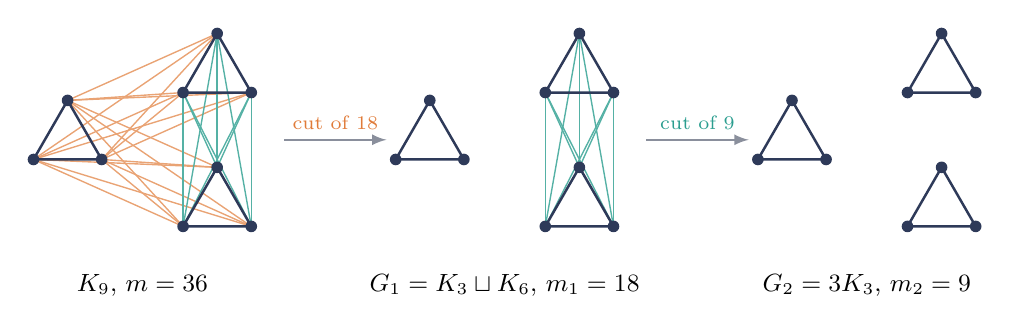
\begin{tikzpicture}[dot/.style={circle, fill=ink, inner sep=0pt, minimum size=4.2pt}]
  \foreach \panel/\xs in {1/0, 2/4.6, 3/9.2} {
    \begin{scope}[xshift=\xs cm]
      \foreach \t/\cx/\cy in {a/0/0, b/1.9/0.85, c/1.9/-0.85}
        \foreach \k/\ang in {1/90, 2/210, 3/330}
          \coordinate (\t\k) at ($(\cx,\cy)+(\ang:0.5)$);
      % level-0 cut: between the triangle a and the six vertices b, c
      \ifnum\panel=1
        \foreach \i in {1,2,3} \foreach \j in {1,2,3} {
          \draw[famB!70, line width=0.5pt] (a\i) -- (b\j);
          \draw[famB!70, line width=0.5pt] (a\i) -- (c\j);
        }
      \fi
      % level-1 cut: between triangles b and c
      \ifnum\panel<3
        \foreach \i in {1,2,3} \foreach \j in {1,2,3}
          \draw[famC!80, line width=0.5pt] (b\i) -- (c\j);
      \fi
      \foreach \t in {a,b,c} {
        \draw[ink, line width=0.9pt] (\t1) -- (\t2) -- (\t3) -- cycle;
        \foreach \k in {1,2,3} \node[dot] at (\t\k) {};
      }
    \end{scope}
  }
  \node[font=\small] at (0.95,-1.85) {$K_9$, $m=36$};
  \node[font=\small] at (5.55,-1.85) {$G_1=K_3\sqcup K_6$, $m_1=18$};
  \node[font=\small] at (10.15,-1.85) {$G_2=3K_3$, $m_2=9$};
  \draw[-latex, soft, line width=0.8pt] (2.75,0) -- node[above, font=\scriptsize, text=famB] {cut of $18$} (4.05,0);
  \draw[-latex, soft, line width=0.8pt] (7.35,0) -- node[above, font=\scriptsize, text=famC] {cut of $9$} (8.65,0);
\end{tikzpicture}
\caption{Iterated parity for $K_9$ (Example~\ref{ex:k9}). The odd differences
must form a cut with $18$ edges, which forces the split $3+6$ (orange). The
differences $\equiv2\pmod4$ must then form a cut of $G_1$ with $9$ edges, which
forces the split of the $K_6$ (green). What is left, three triangles, needs a
cut with $5$ edges at the next level, but every cut of a union of triangles is
even.}
\label{fig:tower}
\end{figure}

For complete graphs the test is easy to run, since every $G_j$ is a disjoint
union of cliques. For $4\le n\le30$ it rules out every $K_n$ except
$n=4,6,11,18,25,27$. Golomb's condition alone, which requires $n$ or $n-2$ to
be a perfect square~\cite{golomb}, also leaves $n=9$ and $n=16$.

\subsection{Other roots of unity}\label{sec:arithmetic}

Fix $q\ge2$ and reduce the labels modulo~$q$. The identity then
says: for each residue $j$ modulo $q$, the number of ordered pairs $(u,v)$ with
$uv\in E$ and $f(u)-f(v)\equiv j\pmod q$ equals the number of integers
$k\in[-m,m]\setminus\{0\}$ with $k\equiv j\pmod q$. Algebraically this is the
identity~\eqref{eq:master} read modulo $z^q-1$, coefficient by coefficient;
equivalently, it holds at \emph{every} $q$th root of unity, including those of
lower order. (Evaluating at a single primitive root loses information when $q$
is composite, so we work with the counts themselves.) For $q=2$
the counts are exactly Golomb's condition.

A labeling must also respect the \emph{capacities} of the interval: at most
$\lfloor(m-j)/q\rfloor+1$ vertices can have labels congruent to $j$, for
$0\le j<q$. Applied to the residue map $v\mapsto f(v)\bmod q$ itself,
together with the capacities, the conditions at any $q\ge2m+1$ are equivalent
to gracefulness, since then a residue determines the label. Without the capacities this fails. For $K_6$ ($m=15$), the residues
$\{0,1,3,8,12,18\}$ modulo $31$ have every nonzero difference exactly once, so
they satisfy the full residue counts at $q=2m+1$, although $K_6$ is not
graceful: the label $18$ lies outside $[0,15]$. (This is a cyclic, not a
perfect, difference set; compare Remark~\ref{rem:windmills}.)

For a graph with a natural vertex partition, such as a complete multipartite
graph, the conditions become quadratic Diophantine equations in the numbers
$n_i(j)$ of labels in part~$i$ congruent to~$j$. Other moduli exclude graphs that parity does not. Complete graphs are a
convenient test: all $K_n$ with $n\ge5$ are excluded anyway, so the question
is only what a fixed modulus can see.

\mgpt\begin{corollary}[a modulus-$3$ obstruction]\label{cor:modthree}
The residue equations modulo $3$ exclude $K_n$ whenever
$n\equiv6,10,11\pmod{12}$.
\end{corollary}

\begin{proof}
Let $x_0,x_1,x_2$ count the labels in the three residue classes and put
$r=m\bmod3$, where $m=\binom n2$. Counting differences divisible by $3$ gives
$\sum_i x_i(x_i-1)=2\lfloor m/3\rfloor$, with $\sum_i x_i=n$.
Consequently, for $u=x_0-x_2$ and $v=x_1-x_2$,
\[
 u^2-uv+v^2=\frac{3\sum_i x_i^2-n^2}{2}=n-r.
\]
The left side is never $2\pmod4$, while the stated congruence classes give
$n-r\equiv2\pmod4$.
\end{proof}

This excludes $K_6$, $K_{11}$ and $K_{18}$, which survive iterated parity,
without a computer search.

\subsection{A parity family of split graphs}

Let $G=K_s\vee\overline K_N$: a clique on $s$ vertices, joined to every vertex of
an independent set of size $N$. Let $S$ and $Y$ be the sums of $(-1)^{f(v)}$
over the clique and over the independent set, and let $\varepsilon=m\bmod2$.
At $z=-1$, the identity~\eqref{eq:master} reads
$\frac12(S^2-s)+SY=-\varepsilon$, that is,
\begin{equation}\label{eq:splitparity}
  S^2+2SY=s-2\varepsilon .
\end{equation}

\mgpt\begin{corollary}[a parity family]\label{cor:splitparity}
If $s\equiv8$ or $10\pmod{16}$, then $K_s\vee\overline K_{2t}$ is not graceful
for any $t\ge1$.
\end{corollary}

\begin{proof}
Since $sN$ is even, $m\equiv\binom s2\pmod2$, so $\varepsilon=0$ when
$s\equiv8$ and $\varepsilon=1$ when $s\equiv10\pmod{16}$. Write $s=4k$ or
$4k+2$; in both cases the right side
of~\eqref{eq:splitparity} is $4k$, and $S$ is even. Put $S=2h$, with $h>0$
after a sign change. Then $h(h+Y)=k$. Here $k\equiv2\pmod4$, so in every
factorization $k=h(h+Y)$ one factor is odd and the other even, and $Y$ is odd.
But $Y$ is a sum of $N=2t$ signs, so it is even.
\end{proof}

For $K_{1,1,1,1,N}=K_4\vee\overline K_N$, \eqref{eq:splitparity} gives
$S=\pm2$ and $Y=0$: $N$ is even, and exactly three clique labels share a
parity. (For odd $N$ this is already Bos\'ak's condition: all degrees are
even and $m=4N+6\equiv2\pmod4$.) The clique vertices have odd degree in Corollary~\ref{cor:splitparity},
so Bos\'ak's condition does not apply there.

Evaluating also at $z=i$ gives a second family. It is the counterpart of
Corollary~\ref{cor:modthree} for the Gaussian integers: there the form
$u^2-uv+v^2$ is the norm of $u+v\omega$, the value at $z=\omega$ of the sum
of $z^{f(v)}$, written in the basis $1,\omega$.

\mgpt\begin{corollary}[a Gaussian-integer obstruction]\label{cor:gauss}
Let $k\ge0$ and $t\ge1$ with $k+t$ odd. Then $K_{8k+6}\vee\overline K_{2t}$
is not graceful. If $k$ is even, it remains not graceful after deleting any
one edge of the clique.
\end{corollary}

\begin{proof}
Put $s=8k+6$ and $N=2t$; then $m=\binom s2+sN\equiv3\pmod4$. Let $C(z)$ and
$X(z)$ be the sums of $z^{f(v)}$ over the clique and over the independent
set. For $|z|=1$ the identity~\eqref{eq:master} reads
\[
 |C(z)|^2-s+2\operatorname{Re}\bigl(C(z)\overline{X(z)}\bigr)
 =\sum_{0<|j|\le m}z^j .
\]
At $z=-1$, with $C(-1)=2p$ and $X(-1)=2q$, this is~\eqref{eq:splitparity}:
$p^2+2pq=2k+1$. So $p$ is odd, which makes the numbers $4k+3\pm p$ of even
and of odd clique labels both even, and $q\equiv k\pmod2$. Hence
$C(i)=2u+2vi$ with $u,v\in\ZZ$. Write $X(i)=x+yi$; then $x$ and $y$ have
the parities of the numbers $t\pm q$ of even and of odd labels in the
independent set, so both are odd. At $z=i$ the right side is $-2$, because
$m\equiv3\pmod4$, and the identity becomes
\[
 u^2+v^2+ux+vy=2k+1 .
\]
But $u(u+x)$ and $v(v+y)$ are even, since $x$ and $y$ are odd.

If an edge $ab$ of the clique is deleted, then $m$ drops by one and the left
side gains the term $-2\operatorname{Re}z^{f(a)-f(b)}$. At $z=-1$, if $f(a)$
and $f(b)$ had the same parity, we would get $p^2+2pq=2k+2$, so $p=2p'$ and
$2p'(p'+q)=k+1$, which is odd. So $f(a)-f(b)$ is odd, the extra term
vanishes at $z=i$, and the same equations as before result.
\end{proof}

The same family also follows from Proposition~\ref{prop:iterated} at level
$j=1$: the parities forced at $z=-1$ make every degree of $G_1$ even, while
$m_1\equiv1\pmod4$. Neither argument reaches $K_6\vee\overline K_4$, which is
not graceful by an exhaustive search: it passes the iterated parity test, and
its residue equations, with capacities, are solvable for every $q\le16$.

\subsection{Limits of parity}\label{sec:cannot}

The residue equations work when few cut sizes are possible, as in a
complete graph, and can fail when $G$ is built from many interchangeable
pieces whose contributions add up to the required cut sizes. In $K_5^{(t)}$ each blade
contributes $0$, $4$ or $6$ edges to Golomb's cut, and these add up to the
required $5t$ for every even~$t$. This is consistent with
Remark~\ref{rem:windmills}: some of these windmills are graceful. For the
complete multipartite graphs $K_{3,3,3}$, $K_{2,2,2,2,2}$, $K_{4,4,4}$ and
$K_{3,4,5}$, all of which are ungraceful by the verification of
Section~\ref{sec:open}, the residue equations are solvable for every
$q\le12$, even together with the capacities.

% ----------------------------------------------------------------
\section{Tool II: positivity on the unit circle}\label{sec:positivity}

\subsection{A warm-up: complete graphs}

Replace each label $x$ by the complex number $e^{itx}$ of modulus~$1$, for a
real parameter $t$ (the \emph{frequency}) to be chosen. For a labeling $f$ we
call the vector $z\in\mathbb C^V$ with entries $z_v=e^{itf(v)}$ the
\emph{phase vector} of $f$ at frequency $t$; its entries are points of the
unit circle. Let $f$ be a graceful labeling of $K_n$. Then
\[
  0\ \le\ \Bigl|\sum_vz_v\Bigr|^2=\sum_{u,v}e^{it(f(u)-f(v))}
  =n+\sum_{u\ne v}e^{it(f(u)-f(v))}=n+D_m(t)-1,
\]
because the differences over ordered pairs $u\ne v$ are $\pm1,\dots,\pm m$, each
once. At the first dip $D_m(t)<-\kappa(2m+1)$, so
$n>1+\kappa(2m+1)=1+\kappa(n^2-n+1)$, which is false for $n\ge5$. So $K_n$ is
not graceful for $n\ge5$, which is Golomb's theorem; this is essentially
R\'edei and R\'enyi's argument. Figure~\ref{fig:phase} shows the case $n=4$, and the failure for $n=5$.
\begin{figure}[ht]
\centering
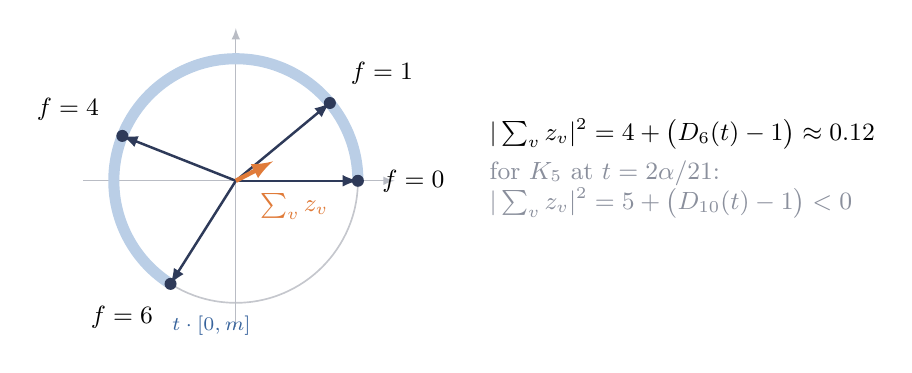
\begin{tikzpicture}[scale=1.55]
  \draw[soft!50, line width=0.6pt] (0,0) circle (1);
  \draw[soft!60, -latex] (-1.25,0) -- (1.3,0);
  \draw[soft!60, -latex] (0,-1.2) -- (0,1.25);
  % arc swept by t*f, 0 <= f <= m
  \draw[famA!35, line width=4pt] (1,0) arc (0:237.65:1);
  \foreach \lab/\ang/\anc in {0/0/west, 1/39.61/south west, 4/158.43/south east, 6/237.65/north east} {
    \draw[-latex, ink, line width=0.9pt] (0,0) -- (\ang:1);
    \fill[ink] (\ang:1) circle (1.4pt);
    \node[anchor=\anc, font=\small] at (\ang:1.12) {$f=\lab$};
  }
  \draw[-latex, famB, line width=1.6pt] (0,0) -- (0.305,0.160);
  \node[famB, font=\small, anchor=north west] at (0.12,-0.02) {$\sum_v z_v$};
  \node[famA!70!ink, font=\scriptsize, anchor=north] at (-0.2,-1.03) {$t\cdot[0,m]$};
  \node[font=\small, align=left, anchor=west] at (2.0,0.1)
    {$|\sum_v z_v|^2=4+\bigl(D_6(t)-1\bigr)\approx0.12$\\[3pt]
     \textcolor{soft}{for $K_5$ at $t=2\alpha/21$:}\\
     \textcolor{soft}{$|\sum_v z_v|^2=5+\bigl(D_{10}(t)-1\bigr)<0$}};
\end{tikzpicture}
\caption{The idea of Tool~II. The labels $0,1,4,6$ of Fig.~\ref{fig:k4} become
the points $z_v=e^{itf(v)}$, here at the first dip $t=2\alpha/13$. Because the differences are $1,\dots,6$, their sum satisfies
$|\sum z_v|^2=n+D_m(t)-1\approx0.12$. Five labels with ten distinct differences
would need, at their own first dip $t=2\alpha/21$,
$|\sum z_v|^2=5+D_{10}(t)-1\approx-0.60$, which is impossible.
This proves that $K_5$ is not graceful.}
\label{fig:phase}
\end{figure}

\subsection{The main theorem}

For a general graph, $|\sum z_v|^2=z^*Jz$, with $J$ the all-ones matrix,
involves all pairs of vertices, while the identity only controls pairs that
are edges. For $K_n$ we have $J=A+I$, where $A$ is the adjacency matrix. The
remedy is to replace $A+I$ by any positive semidefinite matrix that agrees
with $A$ off the diagonal. For a graceful labeling, the phase vector $z_v=e^{itf(v)}$ satisfies
\begin{equation}\label{eq:phase}
  z^*Az=\sum_{uv\in E}2\cos(td_{uv})=D_m(t)-1 ,
\end{equation}
which is below $-\kappa(2m+1)$ at the first dip. So we want matrices $A+\Diag(y)$
that are positive semidefinite with small trace $\sum_vy_v$. Define the
\emph{diagonal completion number} and the \emph{planar energy}
\[
  \mu(G)=\min\Bigl\{\sum_vy_v:\ A+\Diag(y)\succeq0\Bigr\},\qquad
  \gamma_2(G)=\max\bigl\{-z^*Az:\ z\in\mathbb C^{V},\ |z_v|=1\bigr\}.
\]
We call $-z^*Az$ the \emph{energy} of $z$. A complex number of modulus~$1$ is
a unit vector in the plane, so $\gamma_2$ maximizes the energy over unit
vectors in~$\mathbb R^2$; we will see in Section~\ref{sec:exact} that $\mu$ is
the same maximum over unit vectors in any dimension.

\begin{theorem}[positivity]\label{thm:P}
For every graph, $\gamma_2(G)\le\mu(G)$; if $G$ is graceful, then
$\beta_m\le\gamma_2(G)$. In particular $G$ is not graceful if
$\mu(G)\le1+\kappa(2m+1)$, or more generally if $\gamma_2(G)\le1+\kappa(2m+1)$.
\end{theorem}

\begin{proof}
By~\eqref{eq:phase}, the phase vector of a graceful labeling at frequency $t$
has
$-z^*Az=1-D_m(t)$, and maximizing over $t$ gives
$\gamma_2(G)\ge\beta_m$. If $A+\Diag(y)\succeq0$ and $|z_v|=1$, then
$0\le z^*(A+\Diag(y))z=z^*Az+\sum_vy_v$, so $\gamma_2(G)\le\mu(G)$. Finally
$\beta_m>1+\kappa(2m+1)$ by Lemma~\ref{lem:dirichlet}.
\end{proof}

Intuitively, $\mu(G)$ is small when $G$ looks like a union of cliques, and
large when $G$ has a big cut; Section~\ref{sec:exact} makes this exact. For
$K_n$, the matrix $J=A+I$ gives $\mu(K_n)\le n$, and the theorem reduces to the
warm-up.


The parameter $\mu(G)$ is the value of a semidefinite program, and every
feasible $y$ certifies the upper bound $\mu(G)\le\sum_vy_v$. It is convenient to allow certificates whose entries on the
edges lie in $[0,1]$; this gains nothing over $\mu$, but simplifies the
constructions below.

\begin{lemma}[certificates]\label{lem:cert}
Let $M\succeq0$ be indexed by $V(G)$, with $M_{uv}=0$ for distinct
non-adjacent $u,v$ and $0\le M_{uv}\le1$ for every edge. Then
$\mu(G)\le\tr M+2\operatorname{def}(M)$, where $\operatorname{def}(M)=\sum_{uv\in E}(1-M_{uv})$.
\end{lemma}

\begin{proof}
$M+\sum_{uv\in E}(1-M_{uv})(e_u+e_v)(e_u+e_v)^{\mathsf T}$ is positive
semidefinite, equals $A$ off the diagonal, and has trace
$\tr M+2\operatorname{def}(M)$.
\end{proof}

\subsection{First consequences}

Three choices of certificate give the three main corollaries.

\mnew\begin{corollary}[spectral form]\label{cor:spectral}
If $G$ has $n$ vertices, $m$ edges and smallest adjacency eigenvalue $\lmin$,
and $n|\lmin|\le1+\kappa(2m+1)$, then $G$ is not graceful. In particular, a
$k$-regular graph with $\lmin\ge-\kappa k\approx-0.2172\,k$ is not graceful.
\end{corollary}

\begin{proof}
The matrix $A+|\lmin|I$ is positive semidefinite, so
$\mu(G)\le n|\lmin|$. For a $k$-regular graph $m=nk/2$, and
$n|\lmin|\le\kappa nk<1+\kappa(2m+1)$.
\end{proof}

\begin{corollary}[clique packings]\label{cor:cliques}
Suppose $G$ contains edge-disjoint cliques $Q_1,\dots,Q_k$ with
$\sum_i|Q_i|=\sigma$, and $e_0$ edges of $G$ lie in none of them. If
$\sigma+2e_0\le1+\kappa(2m+1)$, then $G$ is not graceful. Consequently:
\begin{enumerate}[label=(\alph*)]
\item $K_n$ is not graceful for $n\ge5$ (Golomb's theorem);
\item the windmill $K_n^{(t)}$ and the disjoint union $tK_n$ are not graceful
  for $n\ge6$;
\item the barbell $B_n$ (two copies of $K_n$ joined by an edge) is not
  graceful for $n\ge6$;
\item $K_n\square P_r$ and $K_n\square C_r$ are not graceful for $n\ge13$,
  for every $r$ ($r\ge3$ for the cycle).
\end{enumerate}
\end{corollary}

\begin{proof}
Apply Lemma~\ref{lem:cert} to $M=\sum_iJ_{Q_i}$, where $J_Q$ is the all-ones
matrix on $Q$: then $\tr M=\sigma$ and $\operatorname{def}(M)=e_0$. For (a), $\sigma=n$,
$e_0=0$, and $n\le1+\kappa(n^2-n+1)$ for $n\ge5$. For (b), $\sigma=tn$, $e_0=0$,
and $tn\le\kappa\,tn(n-1)$ once $n-1\ge1/\kappa\approx4.60$. For (c),
$\sigma=2n$, $e_0=1$, and $2n+2\le1+\kappa(2n^2-2n+3)$ for $n\ge6$. For (d),
with $r$ cliques of size $n$ joined by matchings, $\sigma+2e_0=3rn$ and
$2m=rn(n+1)$ for the cycle, and $\sigma+2e_0=n(3r-2)$ and $2m=rn(n+1)-2n$ for
the path; both inequalities hold once $\kappa(n+1)\ge3$, that is, $n\ge13$.
\end{proof}

\begin{corollary}[dense graphs]\label{cor:dense}
A graph with $n$ vertices and
$m\ge(n^2-1-\kappa)/(2+2\kappa)\approx0.4108\,n^2$ edges is not graceful. In
particular $K_{a_1,\dots,a_r}$ is not graceful when
$\sum a_i^2\le{\frac{\kappa}{1+\kappa}n^2+1}\approx{0.1785\,n^2+1}$, which
includes every complete multipartite graph with $r\ge6$ parts, all of the
same size.
\end{corollary}

\begin{proof}
Take $M=J+L(\overline G)$, where $L(\overline G)$ is the Laplacian of the
complement. It is positive semidefinite, it is $1$ on the edges of $G$ and
$0$ on its non-edges, and $\tr M=n+2\bigl(\binom n2-m\bigr)=n^2-2m$. The
inequality $n^2-2m\le1+\kappa(2m+1)$ is the stated bound. For
$K_{a_1,\dots,a_r}$, $2m=n^2-\sum a_i^2$.
\end{proof}

Corollary~\ref{cor:dense} is the R\'edei--R\'enyi bound for difference
bases~\cite{rr}, with Leech's constant~\cite{leech}, translated into graph
language. A graceful labeling of an $n$-vertex graph gives $n$ integers in
$[0,m]$ whose differences cover $1,\dots,m$; conversely, any such set is the
label set of \emph{some} graceful graph. So the maximum number of edges of a
graceful graph on $n$ vertices is a difference-basis problem (OEIS \href{https://oeis.org/A004137}{A004137}).
For complete multipartite graphs with no part larger than $n/2$, the bound on
$\sum a_i^2$ is exactly what positivity can prove, up to the gap between
$1+\kappa(2m+1)$ and $\beta_m$, even with planar vectors
(Proposition~\ref{prop:maxcut}(c) below); for example $\mu(K_{3,3,3})=27$ and
$\mu(K_{2,2,2,2,2})=20$, both too large.

\subsection{Clique decompositions}

Choosing $M$ to be a weighted sum of all-ones matrices on cliques turns
Theorem~\ref{thm:P} into a purely combinatorial criterion.

\mnew\begin{theorem}[fractional clique decompositions]\label{thm:cliquedec}
Let $\mathcal Q$ be a family of cliques of $G$ with weights $w_Q\ge0$, such that
every edge of $G$ lies in cliques of total weight exactly~$1$. If
$\sum_{Q}w_Q|Q|\le1+\kappa(2m+1)$, then $G$ is not graceful. This holds in
particular when
\[
  \sum_{Q\in\mathcal Q}w_Q\,|Q|\Bigl(|Q|-1-\frac1\kappa\Bigr)\;\ge\;0,
\]
for instance whenever every clique of positive weight has at least $6$
vertices.
\end{theorem}

\begin{proof}
Let $M=\sum_Qw_QJ_Q$. It is positive semidefinite, $M_{uv}=1$ on edges and
$0$ on non-edges, and $\tr M=\sum_Qw_Q|Q|$, so Theorem~\ref{thm:P} applies.
Counting edges with weights gives $2m=\sum_Qw_Q|Q|(|Q|-1)$, so the displayed
inequality says $\tr M\le2\kappa m$, which is less than $1+\kappa(2m+1)$. If
$|Q|\ge6$, then $|Q|-1\ge5>1/\kappa\approx4.60$.
\end{proof}

For $K_n\square P_r$ and $K_n\square C_r$, whose columns are cliques, the
clique-by-clique argument of Corollary~\ref{cor:cliques}(d) is due to
Li~\cite{knuth-err}. The unweighted case
has an older source, in the language of difference sets. If the edges of $G$
split into cliques $Q_1,\dots,Q_t$ and $f$ is a graceful labeling, then the
label sets $f(Q_i)$, each translated to start at~$0$, have positive
differences exactly $1,\dots,m$, whatever the overlaps between the cliques:
they form a \emph{perfect system of difference sets}~\cite{abrham}. Bermond,
Kotzig and Turgeon~\cite{bkt} proved that no perfect system has all of its
sets of one size $n\ge6$, which is the theorem for decompositions into
cliques of one order. Their proof is an elementary rearrangement argument; it
does not reach systems of mixed sizes, which the Dirichlet kernel handles
(for example sets of sizes $6$ and~$4$, or $6$, $5$ and~$5$, by the first
inequality of the theorem). Ma and Yi~\cite{mayi} have recently reproved and
strengthened their result, for families of rulers that all have the same
number of marks, by the one-frequency argument used here, with the same
constant. Bermond, Kotzig and Turgeon state the reduction from clique
decompositions to perfect systems for windmills, and Gallian's
survey~\cite{gallian} states it in general, but as far as we know it has been
applied only to windmills and disjoint unions. The mixed and weighted forms,
the eigenvalue criterion (Corollary~\ref{cor:spectral}), and the families
below appear to be new.

The same reduction turns every nonexistence theorem for perfect systems into
a theorem about graphs. For instance, Bermond, Kotzig and Turgeon showed that
no perfect system consists of two or three sets of size~$4$, or of two sets
of size~$5$~\cite{bkt}. So a graph whose edges split into two or three
copies of $K_4$, or into two copies of $K_5$, is not graceful, however the
cliques meet; three $K_4$'s glued pairwise at three distinct vertices is an
example that is neither a windmill nor a disjoint union. Their argument for
$K_4$'s is the iterated parity of Proposition~\ref{prop:iterated}. With two
or three $K_4$'s, $m=12$ or $18$, and the cut of odd differences must have $6$
or $9$ edges. Each $K_4$ contributes $0$, $3$ or $4$ cut edges, so every $K_4$
is cut as $K_{1,3}$, and $G_1$ consists of two or three edge-disjoint
triangles. Then all degrees of $G_1$ are even, while $m_1=6$ or $9$, which
violates the last sentence of the proposition.

Gallian's survey lists the $K_4$-snakes, chains of $t$ copies of
$K_4$ in which consecutive copies share a vertex, as open. They are not
graceful for $t=2,3$, by the reduction. Dore-Hall reported in 2018 that the
snake with $t=3$ is not graceful and that those with $t=4,5$
are~\cite{dorehall}; one labeling for $t=4$ has blocks $\{2,12,17,20\}$,
$\{0,11,20,24\}$, $\{0,6,22,23\}$, $\{1,3,15,22\}$. A computer search by
the author found one for $t=6$, with blocks $\{0,14,18,34\}$,
$\{0,1,13,36\}$, $\{1,7,22,33\}$, $\{2,9,31,33\}$, $\{2,5,30,35\}$,
$\{3,11,20,30\}$, and we expect the snakes to be graceful for every $t\ge4$.

The number $6$ is the threshold of this criterion for decompositions into
cliques of one size: $5-1<1/\kappa$. Graphs with a few $K_5$'s among larger
cliques can still be excluded by the first inequality of the theorem, but no
statement covering all $K_5$-decompositions is possible by this method, and
indeed some of them are graceful, as the next remark shows.

\begin{remark}[the status of windmills]\label{rem:windmills}
Graceful labelings of windmills come from \emph{perfect difference families}: $t$ sets
of $n$ integers, each containing~$0$, whose positive differences are exactly
$1,\dots,t\binom n2$. Such a family gives a graceful labeling of $K_n^{(t)}$:
identify the $t$ zeros as the hub. A nonzero mark cannot occur in two sets,
since it would repeat a difference from~$0$, so the labels are distinct, and
the edge differences are the given ones. For $n=4$, Ge, Miao and
Sun~\cite{gms} constructed these families for $4\le t\le1000$, and Liu, Feng,
Wang and Zhang constructed them for every $t\ge4$~\cite{lfwz}, settling
Bermond's conjecture: together with~\cite{bkt}, $K_4^{(t)}$ is graceful
exactly when $t\ne2,3$. For $n\ge6$ the windmills are never graceful
(Corollary~\ref{cor:cliques}(b)).

For $n=5$ some windmills are graceful and some are not. $K_5^{(2)}$ is not graceful~\cite{bkt}, and
neither is $K_5^{(4)}$: Kotzig and Turgeon showed by exhaustive elimination
that no perfect family exists for $t=4$~\cite{kt77}, and an exhaustive search by
B.~D.~McKay found no graceful labeling of $K_5^{(4)}$ at all~\cite{mo}. On the
other hand, perfect families with blocks of size~$5$ exist for $t=6,8,10$, and
a recursive construction produces infinitely many more, for example $t=732$
and $t=974$~\cite{mathon}. So $K_5^{(t)}$ \emph{is} graceful for
infinitely many even $t$, and the status of the remaining even $t\ge12$ is open.
Gallian's survey~\cite{gallian} (28th edition, Section~2.4) records
$K_5^{(3)}$ and $K_5^{(4)}$ as graceful, and its summary table also lists
$K_5^{(5)}$; as just explained, none of them is.
\end{remark}

\mnew\begin{corollary}[clique-decomposable graphs]\label{cor:decomp}
\leavevmode
\begin{enumerate}[label=(\alph*)]
\item A graph whose edge set is a disjoint union of cliques, each with at least
  $6$ vertices, is not graceful. In particular, every $K_6$-decomposable graph
  is not graceful.
\item Every edge-transitive graph that contains a $K_6$ is not graceful.
\item \emph{(Parity companion.)} A graph whose edges decompose into an odd
  number of copies of $K_5$, or into $T$ triangles with $T\equiv2,3\pmod4$, is
  not graceful.
\end{enumerate}
\end{corollary}

\begin{proof}
For (a), give each clique weight $1$. For (b), let $c\ge1$ be the number of
copies of $K_6$ containing an edge; by edge-transitivity this does not depend
on the edge. Give every copy of $K_6$ weight $1/c$. For (c), let $r_v$ be
the number of cliques through~$v$. For $K_5$'s the degrees are $4r_v$ and $m=10T\equiv2\pmod4$ when $T$ is odd, so
Corollary~\ref{cor:rosa} applies; for triangles, degrees are $2r_v$ and
$m=3T\equiv1,2\pmod4$ exactly when $T\equiv3,2\pmod4$.
\end{proof}

Cliques that overlap in more than one vertex need a correction on the
overlap. The simplest case is a family introduced by Koh, Rogers, Teo and
Yap~\cite{koh}: let $B(n,r,t)$ be the graph formed by $t$ copies of $K_n$ that
share a common $K_r$. Thus $B(n,1,t)=K_n^{(t)}$ and $B(n,r,1)=K_n$.
Bermond~\cite{bermond} asked which $B(n,r,t)$ are graceful, and Bermond and
Farhi~\cite{bf} showed that they are not when $n$ is sufficiently large
compared with~$r$. Positivity gives an explicit linear threshold, uniform
in~$t$.

\mnew\begin{corollary}[cliques sharing a clique]\label{cor:bnrt}
Let $C=1+1/\kappa\approx5.603$. If $n(n-C)\ge C\,r(r-1)$, then $B(n,r,t)$ is
not graceful for any $t\ge1$. In particular this holds when $n\ge2.4r+6$, and
for $n\ge6,8,10,12,14$ when $r=1,2,3,4,5$.
\end{corollary}

\begin{proof}
Let $R$ be the common $K_r$, and $Q_1,\dots,Q_t$ the copies of $K_n$. Put
$M=\sum_jJ_{Q_j}-(t-1)J_R+(t-1)r\,I_R$. Off the diagonal it is the adjacency
matrix. With $\sigma_R$ and $\sigma_j$ the sums of a vector $x$ over $R$ and
over $Q_j\setminus R$, and using $r\sum_{v\in R}x_v^2\ge\sigma_R^2$,
\[
  x^{\mathsf T}Mx\;\ge\;\sum_j(\sigma_R+\sigma_j)^2-(t-1)\sigma_R^2+(t-1)\sigma_R^2\;\ge\;0 .
\]
Also $\tr M=tn+(t-1)r(r-1)$ and $2m+1=1+r(r-1)+t\bigl(n(n-1)-r(r-1)\bigr)$.
The hypothesis is equivalent to $n+r(r-1)\le\kappa\bigl(n(n-1)-r(r-1)\bigr)$;
multiplying by $t$ and subtracting $r(r-1)$ gives $\tr M<1+\kappa(2m+1)$. If
$n\ge\sqrt C\,r+C$, then $n(n-C)\ge(n-C)^2\ge Cr^2$, and $\sqrt C<2.4$.
\end{proof}

In fact $\gamma_2$ and $\mu$ of $B(n,r,t)$ can be computed exactly.

\mgpt\begin{proposition}[exact values for $B(n,r,t)$]\label{prop:commoncore}
Let $n>r\ge1$, $t\ge1$, $c=n-r$ and $v=r+tc$ (the number of vertices). Then
\[
 \gamma_2(B(n,r,t))=\mu(B(n,r,t))=
 v+\begin{cases}
   (t-1)r^2,&r\le c,\\
   -r^2+2tcr-tc^2,&c\le r\le tc,\\
   t(t-1)c^2,&r\ge tc.
 \end{cases}
\]
\end{proposition}

\begin{proof}
By Proposition~\ref{prop:maxcut}(a) below, $\mu(G)$ is the maximum of
$-\sum_{uv\in E}2\langle x_u,x_v\rangle$ over unit vectors $x_v$ in any
dimension, and $\gamma_2$ is the same maximum in the plane. Let $S$ be the sum
of the $x_v$ over the common $K_r$ and $S_j$ the sum over the rest of the $j$th
copy, with $s=\|S\|\le r$ and $\|S_j\|\le c$. The quantity to maximize is
\[
 v+(t-1)s^2-\sum_j\|S+S_j\|^2\le v+(t-1)s^2-t(s-c)_+^2,
\]
and the right side is largest at $s=\min\{r,tc\}$, which gives the displayed
formula. It is attained in the plane: choose unit complex numbers on the common $K_r$ whose sum has length $s$,
and on each copy unit complex numbers whose sum points the opposite way
with length $\min\{s,c\}$.
\end{proof}

For $n\ge2r$ this reduces to $\gamma_2=\mu=tn+(t-1)r(r-1)$, so the
certificate in the proof of Corollary~\ref{cor:bnrt} is optimal, and better
thresholds for $B(n,r,t)$ will need either the exact test $\mu<\beta_m$ or
information beyond positivity. For
$r=2$ the corollary extends the known fact that $B(n,2,2)$ is not graceful for
$n>5$~\cite{bf,gallian} to all $t$, from $n=8$ on.

Many classical graphs come with a natural partition of their edges into
cliques, and then Theorem~\ref{thm:cliquedec} applies directly. The \emph{Hamming graph} $H(d,q)$ has the words of length
$d$ over a $q$-letter alphabet as vertices, adjacent when they differ in one
coordinate. The \emph{Johnson graph} $J(n,k)$ has the $k$-subsets of an
$n$-set, adjacent when they share $k-1$ elements, and the \emph{Kneser graph}
$K(n,k)$ the same vertices, adjacent when disjoint. The \emph{Grassmann graph}
$J_q(n,k)$ and the \emph{$q$-Kneser graph} $K_q(n,k)$ are their analogues for
$k$-dimensional subspaces of $\mathbb F_q^n$: adjacent when they meet in
dimension $k-1$, respectively only in~$0$. A \emph{partial linear space} is a
set of points with a family of lines such that two points lie on at most one
line; its \emph{collinearity graph} joins two points on a common line.
Generalized quadrangles $\mathrm{GQ}(s,t)$ have $s+1$ points on each line,
nets of order $n$ have $n$ (Latin square graphs are the collinearity graphs of
$3$-nets), and the finite classical polar spaces over $\mathbb F_q$ have
$q+1$.

\mnew\begin{corollary}[line graphs, geometries and subspace graphs]\label{cor:drg}
The following graphs are not graceful:
\begin{enumerate}[label=(\alph*)]
\item the line graph $L(H)$ of any graph $H$, or of any linear hypergraph $H$
  (two edges sharing at most one vertex), with $\delta(H)\ge6$. More generally
  $L(H)$ is not graceful whenever $\sum_vd_v\bigl(d_v-1-\frac1\kappa\bigr)\ge0$,
  the sum running over the vertices of $H$ with $d_v\ge2$.
  This includes the triangular graphs $T(n)=L(K_n)$ with $n\ge7$ and the rook's
  graphs $K_a\square K_b=L(K_{a,b})$ with $a+b\ge12$, and also, by the first
  inequality of Theorem~\ref{thm:cliquedec}, $K_2\square K_9$ and
  $K_3\square K_8$;
\item the collinearity graph of any partial linear space (any two points lie on
  at most one line) in which every line has at least $6$ points. This includes
  generalized quadrangles $\mathrm{GQ}(s,t)$ with $s\ge5$, nets (in particular
  Latin square graphs) of order $n\ge6$, and polar space graphs over
  $\mathbb F_q$ with $q\ge5$. It also includes the block intersection graphs
  of Steiner systems $S(2,k,v)$ with replication number $(v-1)/(k-1)\ge6$;
\item the Hamming graphs $H(d,q)=K_q^{\square d}$ with $q\ge6$, in every
  dimension~$d$;
\item the Johnson graphs $J(n,k)$ ($k\le n/2$) with $n\ge k+5$; in particular
  every $J(n,k)$ with $k\ge5$;
\item every Grassmann graph $J_q(n,k)$, $1\le k\le n-1$, except
  $J_2(2,1)=K_3$ and $J_3(2,1)=K_4$, which are graceful;
\item the Kneser graphs $K(n,k)$ with $n\ge(1+1/\kappa)k\approx5.603\,k$;
\item the $q$-Kneser graphs $K_q(n,k)$ with $k\ge2$, $n\ge2k$, except possibly
  $K_2(4,2)$.
\end{enumerate}
\end{corollary}

\begin{proof}
Items (a)--(d) and (e) for $k\le n-2$ follow from Theorem~\ref{thm:cliquedec}
with a clique partition of the edges.
\begin{itemize}
\item[(a)] For each vertex $v$ of $H$, the edges through $v$ form a clique of
  size $d_v$ in $L(H)$. By linearity each edge of $L(H)$ lies in exactly one of
  these cliques.
\item[(b)] The lines are cliques, and they partition the edges. For a Steiner
  system, the blocks through a point form such a clique.
\item[(c)] The words that agree outside one fixed coordinate form a clique of
  size $q$, and these cliques partition the edges.
\item[(d)] The $k$-sets containing a fixed $(k-1)$-set form a clique of size
  $n-k+1$, and an edge $\{A,B\}$ lies only in the clique of $A\cap B$.
\item[(e)] If $k\le n-2$, the $k$-spaces containing a fixed $(k-1)$-space form
  a clique of size $(q^{n-k+1}-1)/(q-1)\ge q^2+q+1\ge7$, and these cliques
  partition the edges. If $k=n-1$, the graph is complete on
  $(q^n-1)/(q-1)$ vertices, which is at least $5$ except in the two stated
  cases.
\item[(f)] $K(n,k)$ is $\binom{n-k}k$-regular with
  $\lmin=-\binom{n-k-1}{k-1}$, so $|\lmin|/\text{degree}=k/(n-k)$~\cite{bh}; apply
  Corollary~\ref{cor:spectral}.
\item[(g)] $\mathrm{GL}(n,q)$ acts transitively on the edges. Inside
  $\mathbb F_{q^k}^2$, viewed as a $2k$-dimensional space over $\mathbb F_q$,
  the $q^k+1$ subspaces $\{(x,ax)\}$ ($a\in\mathbb F_{q^k}$) and $\{(0,x)\}$
  pairwise meet only in~$0$, so the graph contains $K_{q^k+1}$; when
  $q^k\ge5$, Corollary~\ref{cor:decomp}(b) applies. The only remaining case
  with $k\ge2$ is $q=k=2$. For $n\ge5$, take a $2$-dimensional subspace
  $W\subset\mathbb F_8$; in $W\oplus\mathbb F_8$ the eight subspaces
  $\{(x,ax):x\in W\}$, $a\in\mathbb F_8$, together with any $2$-dimensional
  subspace of $0\oplus\mathbb F_8$, form a $K_9$.
\end{itemize}
For~(a) with $H$ a graph, (c) and~(d), Corollary~\ref{cor:spectral} gives the
same bounds, since the smallest eigenvalues are at least $-2$, $-d$ and $-k$
respectively~\cite{bh}.
\end{proof}

\subsection{Spectral families}

Corollary~\ref{cor:spectral} also reaches graphs without large cliques.

\mnew\begin{corollary}[Paley graphs]\label{cor:paley}
The Paley graph $P(q)$ (vertices $\mathbb F_q$ with $q\equiv1\pmod4$, adjacent
when their difference is a nonzero square) is not graceful for $q\ge37$.
\end{corollary}

\begin{proof}
$P(q)$ is $\frac{q-1}2$-regular with $\lmin=-(1+\sqrt q)/2$~\cite{bh}. The
ratio $(1+\sqrt q)/(q-1)$ is decreasing, and about $0.197<\kappa$ at $q=37$.
\end{proof}

$P(q)$ has even degrees and $m=q(q-1)/4$
edges, so Bos\'ak's condition already excludes $q\equiv5,9\pmod{16}$, including
$q=25$ and $q=37$. The new cases are $q\equiv1,13\pmod{16}$, beginning with
$q=49$ and $q=61$. The smaller graph $P(13)$ is graceful: in the cyclic
order $0,1,\dots,12$ of its vertices, nickgard~\cite{paley13} gives the labels
$0,1,5,39,23,34,13,3,21,7,38,33,24$. For comparison, the hypercubes $H(d,2)$ and the Petersen
graph $K(5,2)$ are graceful~\cite{gallian}; their ratios $|\lmin|/\text{degree}$ are $1$ and $2/3$, far above the shaded
region of Fig.~\ref{fig:map}.

\mnew\begin{corollary}[random regular graphs]\label{cor:random}
For each fixed $d\ge84$, a uniformly random $d$-regular graph on $n$ vertices
($nd$ even) is not graceful with probability tending to~$1$ as $n\to\infty$.
\end{corollary}

\begin{proof}
By Friedman's theorem~\cite{friedman}, in the form for the uniform model
proved by Bordenave~\cite{bordenave}, for every $\epsilon>0$ all eigenvalues
other than $d$ have absolute value at most $2\sqrt{d-1}+\epsilon$ with
probability tending to~$1$. For $d\ge84$, $2\sqrt{d-1}<\kappa d$, and we can
choose $\epsilon$ to fit in between.
\end{proof}

Counting shows that almost all graphs are not graceful~\cite{gallian}, but
it does not reach graphs of fixed degree: there are at most $m!$ graceful
graphs with $m$ edges and no isolated vertices (choose the edge of each
difference $k$ in one of $m-k+1$ positions), and for fixed degree $d$ this
exceeds the number of $d$-regular graphs with $m$ edges.

\mnew\begin{corollary}[more spectral families]\label{cor:spec2}
The following graphs are not graceful:
\begin{enumerate}[label=(\alph*)]
\item every graph with smallest eigenvalue at least $-2$ and average degree at
  least $2/\kappa\approx9.21$;
\item every non-bipartite Ramanujan graph of degree $d\ge84$, that is, every
  $d$-regular graph whose eigenvalues other than $d$ have absolute value at
  most $2\sqrt{d-1}$; for example, the non-bipartite graphs of Lubotzky,
  Phillips and Sarnak~\cite{lps} and of Morgenstern~\cite{morgenstern} of
  degree at least $84$;
\item the polarity graph $\mathrm{ER}_q$~\cite{er62,brown66} for every
  prime power $q\ge23$. Its
  vertices are the points of the projective plane $\mathrm{PG}(2,q)$, with
  $x\sim y$ when $x\ne y$ and $x^{\mathsf T}y=0$. These graphs contain no
  $4$-cycle.
\end{enumerate}
\end{corollary}

\begin{proof}
(a) Here $n|\lmin|\le2n\le\kappa\cdot2m$. (b) Here $\lmin\ge-2\sqrt{d-1}$, and
$2\sqrt{d-1}\le\kappa d$ for $d\ge84$. (c) Let $P$ be the diagonal indicator
of the $q+1$ absolute points ($x^{\mathsf T}x=0$), so that $A'=A+P$ is the
looped matrix. Two distinct points have exactly one common neighbour in $A'$,
so $A'^2=J+qI$, and the eigenvalues of $A'$ are $q+1$ and $\pm\sqrt q$. Hence
$A+P+\sqrt qI\succeq0$, with trace $n\sqrt q+q+1$, where $n=q^2+q+1$ and
$2m=(q+1)(n-1)$. The function $\kappa(q+1)-\sqrt q$ is increasing for
$q\ge23$ and exceeds $0.41$ there, so
$\kappa(2m+1)+1-(n\sqrt q+q+1)\ge n\bigl(\kappa(q+1)-\sqrt q\bigr)-q-\kappa q
>0.41\,q^2-1.22\,q>0$.
\end{proof}

The graphs in~(a) are classified: by the theorem of Cameron, Goethals, Seidel and
Shult~\cite{cgss}, each connected component is a generalized line graph or one
of finitely many exceptional graphs coming from the root system~$E_8$.
In~(c) the certificate has a non-constant diagonal: adding $1$ only at the
$q+1$ absolute points gives trace $n\sqrt q+q+1$, less than the trace
$n(\sqrt q+1)$ of a scalar certificate.

\begin{figure}[ht]
\centering
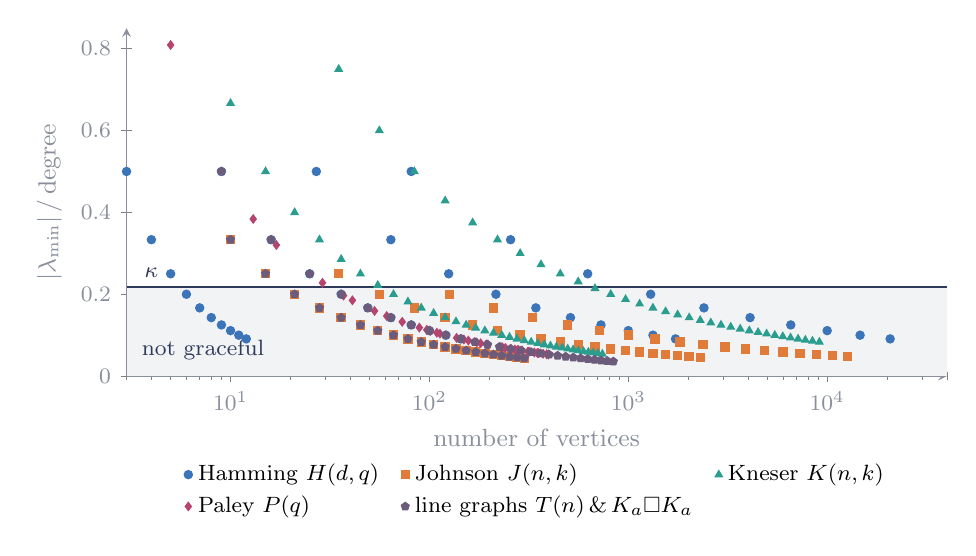
\begin{tikzpicture}
\begin{axis}[
    width=12.0cm, height=6.0cm,
    xmode=log, log basis x=10,
    xmin=3, xmax=40000, ymin=0, ymax=0.85,
    axis lines=left, axis line style={soft},
    tick label style={font=\footnotesize, soft},
    xlabel={number of vertices}, ylabel={$|\lmin|\,/\,\text{degree}$},
    xlabel style={soft, font=\small}, ylabel style={soft, font=\small},
    legend style={font=\footnotesize, draw=none, fill=none,
                  at={(0.5,-0.22)}, anchor=north, /tikz/every even column/.append style={column sep=0.6em}},
    legend columns=3,
    legend cell align=left,
    cycle list={{famA,mark=*},{famB,mark=square*},{famC,mark=triangle*},
                {famD,mark=diamond*},{famE,mark=pentagon*}},
  ]
  \fill[ink!6] (axis cs:3,0) rectangle (axis cs:40000,0.2172);
  \draw[ink, line width=0.9pt] (axis cs:3,0.2172) -- (axis cs:40000,0.2172);
  \node[ink, font=\footnotesize, anchor=south west] at (axis cs:3.3,0.2172) {$\kappa$};
  \node[ink, font=\footnotesize, anchor=south west] at (axis cs:3.2,0.015) {not graceful};
  \pgfplotsset{every axis plot/.append style={only marks, mark size=1.5pt}}
  % hamming
\addplot coordinates {(3,0.5000) (4,0.3333) (5,0.2500) (6,0.2000) (7,0.1667) (8,0.1429) (9,0.1250) (9,0.5000) (10,0.1111) (11,0.1000) (12,0.0909) (16,0.3333) (25,0.2500) (27,0.5000) (36,0.2000) (49,0.1667) (64,0.1429) (64,0.3333) (81,0.1250) (81,0.5000) (100,0.1111) (121,0.1000) (125,0.2500) (144,0.0909) (216,0.2000) (256,0.3333) (343,0.1667) (512,0.1429) (625,0.2500) (729,0.1250) (1000,0.1111) (1296,0.2000) (1331,0.1000) (1728,0.0909) (2401,0.1667) (4096,0.1429) (6561,0.1250) (10000,0.1111) (14641,0.1000) (20736,0.0909)};
% johnson
\addplot coordinates {(10,0.3333) (15,0.2500) (21,0.2000) (28,0.1667) (35,0.2500) (36,0.1429) (45,0.1250) (55,0.1111) (56,0.2000) (66,0.1000) (78,0.0909) (84,0.1667) (91,0.0833) (105,0.0769) (120,0.0714) (120,0.1429) (126,0.2000) (136,0.0667) (153,0.0625) (165,0.1250) (171,0.0588) (190,0.0556) (210,0.0526) (210,0.1667) (220,0.1111) (231,0.0500) (253,0.0476) (276,0.0455) (286,0.1000) (300,0.0435) (330,0.1429) (364,0.0909) (455,0.0833) (495,0.1250) (560,0.0769) (680,0.0714) (715,0.1111) (816,0.0667) (969,0.0625) (1001,0.1000) (1140,0.0588) (1330,0.0556) (1365,0.0909) (1540,0.0526) (1771,0.0500) (1820,0.0833) (2024,0.0476) (2300,0.0455) (2380,0.0769) (3060,0.0714) (3876,0.0667) (4845,0.0625) (5985,0.0588) (7315,0.0556) (8855,0.0526) (10626,0.0500) (12650,0.0476)};
% kneser
\addplot coordinates {(10,0.6667) (15,0.5000) (21,0.4000) (28,0.3333) (35,0.7500) (36,0.2857) (45,0.2500) (55,0.2222) (56,0.6000) (66,0.2000) (78,0.1818) (84,0.5000) (91,0.1667) (105,0.1538) (120,0.1429) (120,0.4286) (136,0.1333) (153,0.1250) (165,0.3750) (171,0.1176) (190,0.1111) (210,0.1053) (220,0.3333) (231,0.1000) (253,0.0952) (276,0.0909) (286,0.3000) (300,0.0870) (325,0.0833) (351,0.0800) (364,0.2727) (378,0.0769) (406,0.0741) (435,0.0714) (455,0.2500) (465,0.0690) (496,0.0667) (528,0.0645) (560,0.2308) (561,0.0625) (595,0.0606) (630,0.0588) (666,0.0571) (680,0.2143) (703,0.0556) (741,0.0541) (816,0.2000) (969,0.1875) (1140,0.1765) (1330,0.1667) (1540,0.1579) (1771,0.1500) (2024,0.1429) (2300,0.1364) (2600,0.1304) (2925,0.1250) (3276,0.1200) (3654,0.1154) (4060,0.1111) (4495,0.1071) (4960,0.1034) (5456,0.1000) (5984,0.0968) (6545,0.0938) (7140,0.0909) (7770,0.0882) (8436,0.0857) (9139,0.0833)};
% paley
\addplot coordinates {(5,0.8090) (13,0.3838) (17,0.3202) (29,0.2280) (37,0.1967) (41,0.1851) (53,0.1592) (61,0.1468) (73,0.1326) (89,0.1186) (97,0.1130) (101,0.1105) (109,0.1059) (113,0.1038) (137,0.0934) (149,0.0892) (157,0.0867) (173,0.0823) (181,0.0803) (193,0.0776) (197,0.0767) (229,0.0708) (233,0.0701) (241,0.0689) (257,0.0665) (269,0.0649) (277,0.0639) (281,0.0634) (293,0.0620) (313,0.0599) (317,0.0595) (337,0.0576) (349,0.0566) (353,0.0562) (373,0.0546) (389,0.0534) (397,0.0528)};
% line
\addplot coordinates {(9,0.5000) (10,0.3333) (15,0.2500) (16,0.3333) (21,0.2000) (25,0.2500) (28,0.1667) (36,0.1429) (36,0.2000) (45,0.1250) (49,0.1667) (55,0.1111) (64,0.1429) (66,0.1000) (78,0.0909) (81,0.1250) (91,0.0833) (100,0.1111) (105,0.0769) (120,0.0714) (121,0.1000) (136,0.0667) (144,0.0909) (153,0.0625) (169,0.0833) (171,0.0588) (190,0.0556) (196,0.0769) (210,0.0526) (225,0.0714) (231,0.0500) (253,0.0476) (256,0.0667) (276,0.0455) (289,0.0625) (300,0.0435) (324,0.0588) (361,0.0556) (400,0.0526) (441,0.0500) (484,0.0476) (529,0.0455) (576,0.0435) (625,0.0417) (676,0.0400) (729,0.0385) (784,0.0370) (841,0.0357)};

  \legend{{Hamming $H(d,q)$}, {Johnson $J(n,k)$}, {Kneser $K(n,k)$}, {Paley $P(q)$}, {line graphs $T(n)$\,\&\,$K_a\square K_a$}}
\end{axis}
\end{tikzpicture}
\caption{Members of several regular families plotted by size and by
$|\lmin|/\text{degree}$.
Corollary~\ref{cor:spectral} makes every regular graph in the shaded region
ungraceful.}
\label{fig:map}
\end{figure}

\subsection{The optimal semidefinite certificate}\label{sec:exact}

The corollaries above each use one convenient certificate. The best possible
certificate has an exact description, because $\mu$ is the dual of a standard
semidefinite program. Let
$\SDP_{\rm MC}(G)=\max\{\sum_{uv\in E}\frac12(1-X_{uv}):X\succeq0,\ X_{vv}=1\}$
be the Goemans--Williamson relaxation of maximum cut~\cite{gw}: a cut is an
assignment of signs $x_v=\pm1$, the edge $uv$ is cut when
$\frac12(1-x_ux_v)=1$, and the relaxation replaces the signs by unit vectors
and $X$ by their Gram matrix.

\mgpt\begin{proposition}[exact form]\label{prop:maxcut}
\leavevmode
\begin{enumerate}[label=(\alph*)]
\item $\mu(G)=\max\{-\langle A,X\rangle:X\succeq0,\ X_{vv}=1\}
  =4\SDP_{\rm MC}(G)-2m$. In particular $\mu(G)\ge4\operatorname{MaxCut}(G)-2m$.
\item If $G$ is vertex-transitive, then $\mu(G)=n|\lmin|$.
\item If $G=K_{a_1,\dots,a_r}$ with $n=\sum a_i$, then
  $\gamma_2(G)=\mu(G)=\sum_ia_i^2-(2\max_ia_i-n)_+^2$.
\end{enumerate}
\end{proposition}

\begin{proof}
Parts (a) and (b) are standard~\cite{dp,mp}; part (c) is new. For~(a), the semidefinite dual of
$\max\{-\langle A,X\rangle:X\succeq0,\ X_{vv}=1\}$ is
$\min\{\sum_vy_v:A+\Diag(y)\succeq0\}=\mu(G)$; both programs are strictly
feasible ($y$ large; $X=I$), so the optima are equal and attained, and
$\sum_{uv\in E}\frac12(1-X_{uv})=\frac m2-\frac14\langle A,X\rangle$ gives the
second form. For~(b), average a feasible $y$ over the automorphism group: the diagonal
becomes constant with the same sum, and $A+cI\succeq0$ exactly when
$c\ge-\lmin$. For~(c), let $S_i$ be the sum of the vectors of $X$'s Gram
factorization over part~$i$. Then $-\langle A,X\rangle=\sum_i\|S_i\|^2-\|\sum_iS_i\|^2$,
and $\|S_i\|\le a_i$. The expression is affine in each $S_i$ separately (its
own square cancels), so the maximum has $\|S_i\|=a_i$, realized by equal
vectors within each part. The smallest possible length of a sum of vectors of
lengths $a_i$ is $(2\max a_i-n)_+$, attained in the plane; so the planar
maximum equals the semidefinite one.
\end{proof}

So the best that a semidefinite certificate can do, with any diagonal and
any frequency, is this: \emph{$G$ is not graceful if
$\SDP_{\rm MC}(G)<(2m+\beta_m)/4$.} Since $\beta_m>1+\kappa(2m+1)$, this
threshold exceeds $\frac12(1+\kappa)m\approx0.6086\,m$. Graphs whose maximum
cut is at least $(2m+\beta_m)/4$ are out of reach even of the planar bound,
because a cut, as a vector of signs $\pm1$, is a vector of unit complex
numbers; for a bipartite graph
$\SDP_{\rm MC}(G)=m$, the largest possible value. This statement concerns
$\mu$, not all of Theorem~\ref{thm:P}: a bound on $\gamma_2$ can be strictly
stronger, as Section~\ref{sec:planar} shows.

Three simple rules transfer certificates from one graph to another; we use
them in Section~\ref{sec:planar}.

\mgpt\begin{lemma}[blocks and edits]\label{lem:blocks}
Let $\eta$ be $\mu$ or $\gamma_2$.
\begin{enumerate}[label=(\alph*)]
\item If subgraphs $F_i$ with weights $w_i\ge0$ cover every edge of $G$ with
  total weight exactly $1$, then $\eta(G)\le\sum_iw_i\eta(F_i)$.
\item If $G$ arises from $H$ by adding $a$ edges and deleting $b$ edges, then
    $|\eta(G)-\eta(H)|\le2(a+b)$.
\item For the independent blowup $F[t]$, obtained by replacing every vertex
  by $t$ independent twins and every edge by a complete bipartite graph,
  $\eta(F[t])=t^2\eta(F)$.
\end{enumerate}
\end{lemma}

\begin{proof}
For $\mu$, add certificates for (a); for (b), an added edge $uv$ costs
$(e_u+e_v)(e_u+e_v)^{\mathsf T}$ and a deleted one
$(e_u-e_v)(e_u-e_v)^{\mathsf T}$, each of trace~$2$. For $\gamma_2$, the energy of a fixed vector $z$ with $|z_v|=1$ splits over
the blocks, and each changed edge changes
it by at most~$2$. For (c), sum the vectors in each twin class to get vectors
$S_v$ of length at most $t$. The energy is affine in each $S_v$ separately, so
its maximum has $\|S_v\|=t$, realized by equal vectors within each class;
this works in the plane and in any dimension.
\end{proof}

Three further remarks bound what refinements of positivity can achieve.

\emph{Averaging frequencies.} One could replace the function $x\mapsto e^{itx}$ by any
positive definite function $\varphi$ on~$\ZZ$ with $\varphi(0)=1$, since the matrix
$\bigl(\varphi(f(u)-f(v))\bigr)_{u,v}$ is then positive semidefinite. By
the Herglotz--Bochner theorem~\cite{rudin}, $\varphi(x)=\int e^{itx}\,d\nu(t)$ for a probability measure~$\nu$, and the identity becomes
$\sum_{uv\in E}2\operatorname{Re}\varphi(d_{uv})=\int(D_m(t)-1)\,d\nu(t)$, an
average of the single-frequency case; it can never do better than the best
single frequency. Bernshteyn and Tait~\cite{bt} beat Leech's constant for
difference bases only by using several Fourier coefficients of one measure
jointly. A similar gain for graphs would need constraints that tie different
frequencies together.

\emph{Abelian Cayley graphs.} For a Cayley graph of an abelian group, the
eigenvector for $\lmin$ can be taken to be a character, all of whose entries
have modulus~$1$, so $\gamma_2=\mu=n|\lmin|$. This settles the unrestricted
planar optimization for Paley, Hamming and rook's graphs and for $K_n$, but not refinements that
remember that the entries of an actual phase vector lie on a finite grid and, at the first dip, on
an arc of length about $\alpha<2\pi$.

\emph{Adding parity.} Knowing which edges have even differences, one might
give them weight~$1$ and give the odd ones weight $c\in[-1,1]$. The right side
then becomes $\frac{1+c}2\,D_m(t)+\frac{1-c}2\,D_m(t+\pi)-1$, a convex
combination of two translates of $D_m-1$, whose minimum is no lower. So the
kernel side gains nothing; any gain would have to come from the graph side,
from certificates for the reweighted matrix, which depends on the unknown
cut. We have not found a way to exploit this.

\subsection{The planar refinement}\label{sec:planar}

The vectors $z_v=e^{itf(v)}$ are complex
numbers of modulus~$1$, while $\mu(G)$ allows unit vectors in any dimension,
and Theorem~\ref{thm:P} already records the stronger inequality
$\gamma_2(G)\ge\beta_m$. The following lemma is one way to
use it: it bounds the projection onto the least eigenspace of a vector whose
entries have modulus~$1$.

\mgpt\begin{lemma}[projection onto the least eigenspace]\label{lem:projection}
Let $\theta>\lmin$ be the second smallest distinct adjacency eigenvalue of
$G$, let $U\subseteq\mathbb C^V$ be the eigenspace of~$\lmin$, and put
$\Lambda(U)=\max\{\|w\|_1:w\in U,\ \|w\|_2=1\}$. Then
\[
 \gamma_2(G)\le(\theta-\lmin)\Lambda(U)^2-\theta n.
\]
\end{lemma}

\begin{proof}
Let $P$ be the orthogonal projection onto $U$. If $|z_v|=1$ for all $v$, then
$\|z\|_2^2=n$ and $\|Pz\|_2=\max_{w\in U,\,\|w\|_2=1}|w^*z|\le\Lambda(U)$. The
spectral decomposition gives $z^*Az\ge\lmin\|Pz\|_2^2+\theta(n-\|Pz\|_2^2)$.
\end{proof}

\mgpt\begin{theorem}[a planar bound for $K(11,2)$]\label{thm:kg}
Let $H=K(11,2)$, the Kneser graph on the $55$ pairs from an $11$-set. It is
$36$-regular with $990$ edges, $\mu(H)=440$, and
\[
  \gamma_2(H)\le\frac{26409}{64}=412.640625.
\]
\end{theorem}

The bottom eigenspace of $K(11,2)$ consists of the vectors whose entry at a
pair $\{i,j\}$ is $a_i+a_j$, with $\sum_ia_i=0$. The proof bounds
$\sum_{i<j}|a_i+a_j|$ by $173/8$ when $\sum_ia_i=0$ and $\sum_i|a_i|^2=1$, using the relation
between the largest $|a_i+a_j|$ and the fourth moment $\sum_i|a_i|^4$; then
$\Lambda(U)\le173/24$, and Lemma~\ref{lem:projection} with $\lmin=-8$ and
$\theta=1$ gives the theorem. The details are in Appendix~\ref{app:kg}.

The max-cut of $K(n,2)$ and its eigenvalue bound are
classical~\cite{pt,mp}, and the gap between
rank-constrained and unconstrained semidefinite programs is studied
in~\cite{bov}; we know of no earlier bound on the planar value of a
Kneser graph. Theorem~\ref{thm:kg} gives an explicit margin, and hence the
following family.

\mgpt\begin{corollary}[planar families]\label{cor:kg}
Let $H_b$ be $K(11,2)$ with any $b\in\{0,\dots,7\}$ edges deleted. Every
$H_b$ is not graceful, and neither is any graph whose edges have a
fractional decomposition into such graphs, or any independent blowup of
such a graph. On every $H_b$ and each of its independent blowups, every
semidefinite certificate fails, at every frequency.
\end{corollary}

\begin{proof}
Theorem~\ref{thm:kg} and Lemma~\ref{lem:blocks}(b) give
$\gamma_2(H_b)\le26409/64+2b$. Since $\kappa$ is the maximum of
$-\sin x/x$, and $0<\frac32\pi-\frac92<\frac3{14}$, the inequality
$\cos x>1-x^2/2$ gives $\kappa\ge\frac29\cos(\frac32\pi-\frac92)>
\frac{383}{1764}$. Hence
\[
 2\kappa(990-b)-\gamma_2(H_b)
 >\frac{383}{882}(990-b)-\frac{26409}{64}-2b\ge\frac{6143}{28224}>0,
\]
so $\gamma_2(H_b)<2\kappa|E(H_b)|<1+\kappa(2m+1)$. These inequalities add
over a fractional decomposition, by Lemma~\ref{lem:blocks}(a), and both sides
scale by $t^2$ under blowups, by Lemma~\ref{lem:blocks}(c);
Theorem~\ref{thm:P} applies in each case.

For the semidefinite comparison, let $B$ be the incidence matrix of $K_{11}$
and put $X_0=\frac{11}{18}B^{\mathsf T}(I-\frac1{11}J)B$. It is positive
semidefinite with unit diagonal and has entry $-2/9$ on each edge of $H$; it
stays feasible after edges are deleted, so
$\mu(H_b)\ge440-\frac49b\ge\frac{3932}9>436$. Lemma~\ref{lem:betabound} gives
$\beta_{990-b}\le1+525\cdot1981/2399<436$ for $0\le b\le7$, and the same
comparison holds after a blowup by $t$, since $\mu$ scales by $t^2$ while
$\beta_{t^2m}/t^2\le(1+\frac{525}{2399})/t^2+\frac{1050m}{2399}<436$.
\end{proof}

The same margin also allows edge additions: a graph obtained from
$K(11,2)$ by adding $a$ edges and deleting $b$ edges is not graceful whenever
$44192a+68704b\le487070$, for instance after any eleven additions. The graph
$K(11,2)$ itself is excluded by Bos\'ak's condition ($36$ is even and
$990\equiv2\pmod4$). For $1\le b\le7$ it excludes $H_b$ only when the deleted
edges form an even subgraph (every vertex meeting an even number of them) and
$990-b\equiv1,2\pmod4$, that is, only for $b=4,5$ (for example, a deleted
$4$-cycle or $5$-cycle). It says nothing about $H_1$ and $H_2$, which have
vertices of odd degree, nor about $H_3$, $H_6$ and $H_7$, whose numbers of
edges are $\equiv0,3\pmod4$.

% ----------------------------------------------------------------
\section{Tool III: the interval}\label{sec:interval}

Tool~III uses the bounded span of the labels, which are distinct integers
in $[0,m]$. This forces the labels of a dense subgraph to span a long interval: a clique $K_r$ has $\binom r2$
distinct differences among its labels, so those labels must spread over an
interval of length at least $\binom r2\approx r^2/2$, and in fact of length
about $r^2$ (Theorem~\ref{thm:core} below); a graph with fewer than about
$r^2$ edges cannot provide that interval. For a graph $H$, let $\ell(H)$ be
the smallest span $\max f-\min f$ of an injective integer labeling of $H$ whose
edge differences are all distinct (they need not be $1,\dots,|E(H)|$). Then
\begin{equation}\label{eq:span}
  H\subseteq G,\ G\text{ graceful}\quad\Longrightarrow\quad\ell(H)\le|E(G)| .
\end{equation}
For $H=K_r$, $\ell(H)$ is the length of the shortest $r$-mark Golomb ruler. Ungracefulness of $H$ says nothing about its supergraphs, but a lower bound
on $\ell(H)$ excludes every graph with fewer than $\ell(H)$ edges that
contains~$H$.

\mgpt\begin{theorem}[dense core]\label{thm:core}
Suppose $G$ has $m$ edges and contains a subgraph $H$ on $r$ vertices that
misses at most $p$ of the $\binom r2$ pairs. For an integer $1\le h\le r-1$,
put $T=hr-\frac{h(h+1)}2-p$. If $T>0$ and $G$ is graceful, then
\[
  m\ \ge\ \frac{T(T+1)+2p}{h(h+1)}+\frac{2(h-1)}3 .
\]
If $H=K_r$ and $r\ge2h$, the bound improves to
$m\ge\frac{T(T+1)}{h(h+1)}+\frac{h^2-1}3$.
\end{theorem}

\begin{proof}
Order the labels on $H$ as $a_1<\dots<a_r$, all in $[0,m]$, and put
$S_h=\sum_{j=1}^h\sum_{i=1}^{r-j}(a_{i+j}-a_i)$. There are
$P=hr-h(h+1)/2$ pairs whose indices differ by at most $h$; let $p'\le p$ of
them be non-edges. The other $P-p'$ have distinct positive differences, and
each non-edge has length at least one, so
$S_h\ge\frac{(P-p')(P-p'+1)}2+p'\ge\frac{T(T+1)}2+p$. For fixed $j$, the
inner sum splits into $j$ telescoping chains by residue of $i$ modulo $j$
(Fig.~\ref{fig:core}); since the labels are distinct integers,
\[
 \sum_{i=1}^{r-j}(a_{i+j}-a_i)=\sum_{i=r-j+1}^ra_i-\sum_{i=1}^ja_i
 \le j(a_r-a_1)-j(j-1)\le jm-j(j-1).
\]
Summing over $j\le h$ gives $S_h\le\frac{h(h+1)}2m-\frac{(h-1)h(h+1)}3$, which
proves the first bound.

For a clique, write $S_h=\sum_ig_iw_i$ with gaps $g_i=a_{i+1}-a_i$, where
$w_i$ is the number of chosen pairs whose interval contains the $i$th gap. Interior
gaps have weight $W=h(h+1)/2$; the first $h-1$ gaps and the last $h-1$ have
deficits $W-w_i=\binom{h-i+1}2$, $1\le i\le h-1$, each value occurring twice.
These $2(h-1)$ gaps are distinct edge differences, so
$\sum_i(W-w_i)g_i\ge\sum_{j=1}^{h-1}(4j-1)\binom{h-j+1}2=\frac{h(h-1)(h+1)^2}6$,
by giving the smallest gaps to the largest deficits. Thus
$S_h\le Wm-\frac{h(h-1)(h+1)^2}6$, and dividing by $W$ gives the extra
$\frac{h^2-1}3$.
\end{proof}

\begin{figure}[ht]
\centering
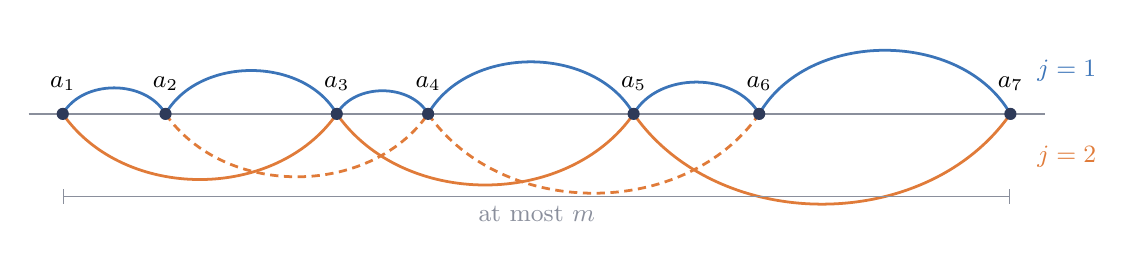
\begin{tikzpicture}[x=1.45cm]
  \draw[soft, line width=0.6pt] (-0.3,0) -- (8.6,0);
  \foreach \i/\x in {1/0, 2/0.9, 3/2.4, 4/3.2, 5/5.0, 6/6.1, 7/8.3} {
    \coordinate (a\i) at (\x,0);
  }
  % j = 1: consecutive pairs, above
  \foreach \i/\j in {1/2, 2/3, 3/4, 4/5, 5/6, 6/7}
    \draw[famA, line width=1.0pt] (a\i) to[out=60, in=120] (a\j);
  % j = 2: two chains below
  \foreach \i/\j in {1/3, 3/5, 5/7}
    \draw[famB, line width=1.0pt] (a\i) to[out=-55, in=-125] (a\j);
  \foreach \i/\j in {2/4, 4/6}
    \draw[famB, line width=1.0pt, densely dashed] (a\i) to[out=-55, in=-125] (a\j);
  \foreach \i in {1,...,7} {
    \fill[ink] (a\i) circle (2.2pt);
    \node[font=\small, above=5pt] at (a\i) {$a_{\i}$};
  }
  \node[famA, font=\small, anchor=west] at (8.45,0.55) {$j=1$};
  \node[famB, font=\small, anchor=west] at (8.45,-0.55) {$j=2$};
  \draw[soft, |-|] (0,-1.05) -- node[below, font=\small, text=soft] {at most $m$} (8.3,-1.05);
\end{tikzpicture}
\caption{The counting behind Tool~III, for $r=7$ and $h=2$. The arcs join
labels whose indices differ by at most $h$; at least $T$ of them are edges, whose lengths are distinct and so add up
to at least $1+2+\cdots+T$. But for each $j$ the
arcs of index distance $j$ form $j$ chains (solid and dashed below), each
lying inside $[a_1,a_r]$, so their total length is at most $j\,m$.}
\label{fig:core}
\end{figure}

Taking $h$ of order $\sqrt r$ gives $\ell(K_r)\ge r^2-O(r^{3/2})$, the classical
Erd\H{o}s--Tur\'an--Lindstr\"om estimate~\cite{et,lindstrom}; much sharper bounds
are known for Golomb rulers~\cite{cho}. That the clique labels of a graceful
graph form a Golomb ruler is folklore (see~\cite{gallian}), and the
asymptotic form of Theorem~\ref{thm:core} for dense subgraphs is due to
Ferrara, Kohayakawa and R\"odl~\cite{fkr} and to Bollob\'as and
Pikhurko~\cite{bp}, in the language of integer sets with prescribed distinct
differences. What Theorem~\ref{thm:core} adds is an explicit inequality,
usable for specific $r$, and its application to gracefulness. So a graph containing $K_r$ with at most
$(1-\varepsilon)r^2$ edges is not graceful once $r$ is large, which allows
almost $r^2/2$ edges beyond the clique's own. The bound depends only on $m$, so the extra edges may be placed
arbitrarily. In the next corollary they are pendant leaves, which create a
large cut and absorb the parity constraints; neither positivity nor
iterated parity excludes these graphs (Proposition~\ref{prop:missed}).

\mgpt\begin{corollary}[cliques with many leaves]\label{cor:leaves}
\leavevmode
\begin{enumerate}[label=(\alph*)]
\item For $r\ge46$, the graph obtained from $K_r$ by attaching
  $\lfloor r^2/4\rfloor$ pendant leaves to one vertex is not graceful.
\item For even $r\ge102$, the graph obtained from $K_r$ by deleting a perfect
  matching and attaching $r^2/4$ pendant leaves to one vertex is not graceful.
\end{enumerate}
\end{corollary}

\begin{proof}
(a) Here $m\le\frac34r^2-\frac r2$. Take $h=6$, $T=6r-21$:
$\frac{(6r-21)(6r-20)}{42}+\frac{35}3-\bigl(\frac34r^2-\frac r2\bigr)
=\frac{9r^2-450r+1820}{84}>0$ for $r\ge46$.
(b) Here $p=r/2$ and $m=\frac34r^2-r$. Take $h=13$, $T=(25r-182)/2$:
$\frac{T(T+1)}{182}-m=\frac{79r^2-8322r+32760}{728}>0$ for $r\ge102$
(dropping the other, nonnegative terms of the bound).
\end{proof}

\mgpt\begin{lemma}[leaves absorb the parity constraints]\label{lem:leaves-parity}
Let $H$ be a graph on $r$ vertices, let $v$ be a vertex of $H$, and let $G$ be
obtained by attaching leaves to $v$. If $G$ has $m\ge r^2/2$ edges, then $G$ passes the iterated parity test.
\end{lemma}

\begin{proof}
Give the vertices of $H$ the auxiliary labels $0,\dots,r-1$, with $0$ at $v$.
For $q=2^j$, let $c_j$ be the number of edges of $H$ whose difference has
$2$-adic valuation $j$. The $q$ residue classes of $\{0,\dots,r-1\}$ have
sizes $r_a\in\{k,k+1\}$, where $r=kq+s$ with $0\le s<q$, so
$c_j\le\sum_a\lfloor r_a^2/4\rfloor\le\lfloor r^2/(4q)\rfloor$: a direct
computation shows that $r^2/(4q)-\sum_a\lfloor r_a^2/4\rfloor$ equals
$s^2/(4q)$ when $k$ is even and $(q-s)^2/(4q)$ when $k$ is odd. The test at
level $j$ requires $o_j=\lceil\lfloor m/q\rfloor/2\rceil\ge\lfloor
m/(2q)\rfloor\ge c_j$ edges of valuation $j$. Give $o_j-c_j$ of the leaves labels of valuation $j$ (the labels need not
be distinct); this uses all the leaves, since $\sum_jo_j=m$ and
$\sum_jc_j=|E(H)|$. The cuts defined by the successive binary digits then
have exactly the required sizes.
\end{proof}

The auxiliary labels need not lie in $[0,m]$, so the lemma concerns the
parity test, not the residue tests with capacities.

\mgpt\begin{proposition}[what parity and positivity miss]\label{prop:missed}
Neither iterated parity nor positivity can prove Corollary~\ref{cor:leaves}: both
families pass the iterated parity test, and
satisfy $\mu(G)\ge\gamma_2(G)>\beta_m$.
\end{proposition}

\begin{proof}
Both families have $m\ge r^2/2$, so Lemma~\ref{lem:leaves-parity} applies.
Split $K_r$ into two halves, and put the leaves on the side opposite to
the vertex that carries them. In~(a)
this cut has $B=2\lfloor r^2/4\rfloor\ge2m/3$ edges, and in~(b) at least
$r^2/2-r/2\ge2m/3$. Its $\pm1$ vector has energy $4B-2m$, so
$\gamma_2(G)\ge4B-2m\ge2m/3$. On the other hand, $D_m(t)<0$ forces
$t\ge2\pi/(2m+1)$ on $[0,\pi]$, so $\beta_m\le1+\csc\frac\pi{2m+1}
\le1+\frac{2m+1}\pi+\frac\pi{2m+1}<\frac{2m}3$ for $m\ge100$, which holds in both families.
\end{proof}

The same counting applies to several cliques at once.

\mgpt\begin{corollary}[the interval for clique packings]\label{cor:packing}
Suppose $G$ has $m$ edges and contains $t$ edge-disjoint copies of $K_r$. For
an integer $1\le h\le r-1$ put $T=hr-\frac{h(h+1)}2$. If $G$ is graceful, then
\[
  m\ \ge\ \frac{T(tT+1)}{h(h+1)},
\]
and if $r\ge2h$, then
\[
  m\ \ge\ \frac{T(tT+1)}{h(h+1)}+\frac{(h-1)(th+1)}3 .
\]
\end{corollary}

\begin{proof}
Run the proof of Theorem~\ref{thm:core} in each copy. The $tT$ chosen pairs are
all edges, of the same copy or of different ones, so their differences are
distinct: their sum is at least $tT(tT+1)/2$ and at most $tWm$, with
$W=h(h+1)/2$. For the refinement, the deficits $\binom{h-j+1}2$,
$1\le j\le h-1$, occur twice in each copy, and the corresponding $2t(h-1)$
boundary gaps are distinct edge differences. Giving the smallest gaps to the
largest deficits, the total deficit is at least
$\sum_{j=1}^{h-1}t(4tj-2t+1)\binom{h-j+1}2=\frac{th(h-1)(h+1)(th+1)}6$.
Subtract this from $tWm$ and divide by $tW$.
\end{proof}

For example, $r=20$ and $h=4$ give $m\ge249t+\frac92$: $t$ edge-disjoint
copies of $K_{20}$ together with at most $59t+4$ further edges, arranged in
any way, never form a graceful graph. Shifting the labels of each copy to start at~$0$ turns the copies
into a \emph{difference triangle set}~\cite{cc}: $t$ sets of $r$ integers, each
containing~$0$, with all differences within the sets distinct; its
\emph{scope} is the largest element. Conversely, a windmill with pendant edges
at its hub realizes any difference triangle set, one pendant edge for each
missing difference. So the least number of edges of a graceful graph
containing $t$ edge-disjoint copies of $K_r$ is exactly the least scope of a
difference triangle set with $t$ rows of $r$ marks, and the first bound of
Corollary~\ref{cor:packing} is the classical counting bound for that
problem~\cite{cc},
translated into graph language. Per copy of $K_r$, positivity
(Corollary~\ref{cor:cliques}) forces about $r(r-2)/(2-2\kappa)\approx0.64\,r^2$
edges, and Corollary~\ref{cor:packing} forces $r^2-O(r^{3/2})$. For large
$t$, positivity is the stronger of the two for $6\le r\le11$, and the interval
from $r=12$ on: with $h=3$ the interval gives $\frac34(r-2)^2+2$ per copy,
which is $77$ at $r=12$, against $76.65$ from positivity. At $r=6$
positivity gives $15.33\,t$ edges, more than Shearer's linear-programming
bound $(91t+6)/6$ for difference triangle sets~\cite{shearer}. Ma and Yi~\cite{mayi} obtain the same positivity constant for difference
triangle sets; their counting bound, which lacks the boundary-gap term,
overtakes positivity only from $r=14$.

% ----------------------------------------------------------------
\section{History and provenance}\label{sec:provenance}

\subsection*{Classical background}
\begin{itemize}
\item Graceful labelings ($\beta$-valuations) are due to Rosa~\cite{rosa65,rosa}.
  The parity condition (Corollary~\ref{cor:rosa}) is due to J.~Bos\'ak; Rosa
  credits it to him in his 1965 thesis~\cite[p.~17]{rosa65}, and published it
  in~\cite{rosa}. The refinement in Corollary~\ref{cor:knuthparity} appears in
  Section~7.2.2.3 of Knuth's \emph{The Art of Computer Programming},
  Volume~4, Fascicle~7~\cite{knuth-pre}. The application of the parity condition to the
  windmills $K_5^{(t)}$ comes from a MathOverflow answer by the
  author~\cite{mo}.
\item The name, the partition condition, and the theorem that $K_n$ is
  graceful only for $n\le4$ are due to Golomb~\cite{golomb}.
\item The analytic step of Tool~II, evaluating the identity at the first dip
  of the Dirichlet kernel, is due to R\'edei and R\'enyi~\cite{rr}, with
  Leech's constant $\kappa$~\cite{leech}; Bernshteyn and Tait improved the
  difference-basis constant using coupled Fourier information~\cite{bt}. They
  worked on difference bases, not graphs. The max-cut relaxation is Goemans and
  Williamson's~\cite{gw}.
\item The ordered-difference argument of Tool~III goes back to
  Lindstr\"om's bound for Sidon sets~\cite{lindstrom}.
\item Windmills $K_n^{(t)}$ with $n\ge6$ were shown ungraceful by Koh,
  Rogers, Teo and Yap~\cite{koh}, and disjoint unions $tK_n$ ($t\ge2$) by
  Kotzig and Turgeon~\cite{kotzig}. Bermond, Kotzig and Turgeon~\cite{bkt}
  proved that no perfect system of difference sets has all its sets of one
  size $n\ge6$, which is Theorem~\ref{thm:cliquedec} for cliques of one
  order; they also used the case $j=1$ of Proposition~\ref{prop:iterated} and
  excluded $K_5^{(2)}$. Kotzig and Turgeon excluded perfect families for
  $K_5^{(4)}$~\cite{kt77}, and Mathon recorded perfect families of size-$5$ blocks for $t=6,8,10$ and
a recursive construction~\cite{mathon}.
\item The complete multipartite conjecture is Beutner and Harborth's~\cite{beutner}.
  The graphs $B(n,r,t)$ are due to Koh, Rogers, Teo and Yap~\cite{koh}, the
  question of their gracefulness to Bermond~\cite{bermond}, and the
  non-explicit bound to Bermond and Farhi~\cite{bf}.
\end{itemize}

\subsection*{Recent work}
In 2026 Shisheng Li applied the R\'edei--R\'enyi argument to graphs built from
cliques, with one sum per clique. He proved that $K_n\square P_4$ is
ungraceful for $n\ge11$, and that $K_n\square P_r$ and $K_n\square C_r$ are
ungraceful for $n\ge13$; this was reported by Knuth~\cite{knuth-err}, whose
note~\cite{knuth-coups} gives the background on these graphs. Ma and
Yi~\cite{mayi} have used the same Dirichlet-kernel obstruction for families
of Golomb rulers. Liu, Feng, Wang and Zhang settled the four-clique
windmills~\cite{lfwz}.

\subsection*{Results new here, and how they were found}
Results marked \new\ or \gpt\ are new as far as we know; several are short
deductions, and we would be glad to hear of earlier appearances. The text was written by Claude Opus~5.5 (Anthropic),
at the direction of the author; some passages of version~2 are adapted from a
revision by GPT-6 Pro. The barbell
theorem (Corollary~\ref{cor:cliques}(c)) comes from an earlier note written in
the same collaboration, which started this project. A targeted search for prior statements of
the main results found the antecedents cited in the text: Li's clique argument
and the theorem of Bermond, Kotzig and Turgeon on perfect systems for
Tool~II, the asymptotic dense-subgraph bounds of~\cite{fkr,bp} for
Tool~III, and classical max-cut and rank-constrained semidefinite work for the
planar refinement; several older proceedings papers (notably~\cite{bermond,bf})
could not be checked in full. Results marked \new\ were found by Claude in
this collaboration. Results marked \gpt\ were found by
GPT-6 Pro (OpenAI), most of them in a referee report on an earlier draft, which
also corrected the status of the windmills $K_5^{(t)}$ and suggested using
$\kappa$ throughout. The author has not checked every proof in detail.
The finite and numerical claims of the paper are checked by Python scripts
at \url{https://github.com/boonsuan/tools}, in exact rational arithmetic
wherever a proof uses them; their README lists which script checks which
result. The search mentioned
in Section~\ref{sec:open} is author-reported.

Version~2 incorporates a revision by GPT-6 Pro. It corrected four points of
version~1: the description of de Bruijn's tiles, the status of $P(13)$, which
is graceful~\cite{paley13}, the credit for the $K_4$-snakes~\cite{dorehall},
and the scope of the statement that the max-cut relaxation describes what
positivity can prove, which applies to $\mu$ and not to $\gamma_2$. It also
contributed the results marked~\gpt\ that are new in this version: the
modulus-$3$ family, the exact energies of $B(n,r,t)$, the projection lemma,
Theorem~\ref{thm:kg} and Corollary~\ref{cor:kg} for $K(11,2)$, the
boundary-gap terms in Theorem~\ref{thm:core} and
Corollary~\ref{cor:packing}, and the leaf lemma. Corollary~\ref{cor:gauss}
was found by GPT-6 Pro later, after the author suggested evaluating the
identity at other points. The verification scripts
were written by Claude for version~2, partly adapted from scripts in that
revision.

% ----------------------------------------------------------------
\section{Open problems}\label{sec:open}

\begin{enumerate}
\item \emph{The Beutner--Harborth conjecture.} Beutner and
  Harborth~\cite{beutner} gave graceful labelings of $K_{1,m,n}$, $K_{2,m,n}$
  and $K_{1,1,m,n}$, and conjectured that these, together with $K_{m,n}$, are
  the only graceful complete multipartite graphs; it has been verified for up
  to $23$ vertices~\cite{gallian} (and, by our own search, $26$). The tools
  here settle every complete multipartite graph with
  $\sum a_i^2\le\frac\kappa{1+\kappa}n^2+1$, and by
  Proposition~\ref{prop:maxcut}(c) that is exactly the reach of positivity when
  no part exceeds $n/2$; for example $\mu(K_{3,3,3})=27$, and
  $\mu(K_{2,2,2,2,2})=20>\beta_{40}\approx18.6$. Residues alone also fail for
  $K_{3,3,3}$, $K_{2,2,2,2,2}$, $K_{4,4,4}$ and $K_{3,4,5}$
  (Section~\ref{sec:cannot}). Since $K_{4,4,4}$ and $K_{5,5,5}$ have
  $\rho$-labelings (Section~\ref{sec:dictionary}), a proof must use that the labels lie in $[0,m]$, not only their residues
  modulo $2m+1$, and Tool~III as stated does not exclude these graphs.
\item Prove that $K_{1,1,1,1,N}=K_4\vee\overline K_N$, the simplest open case
  of the Beutner--Harborth conjecture, is not graceful for any $N\ge1$.
  Parity forces $N$ to be even (Section~\ref{sec:parity}), and positivity
  cannot help, since $\mu=\gamma_2=8N-12$ for $N\ge4$
  (Proposition~\ref{prop:maxcut}(c)). The interval does constrain a labeling. Normalize so that $0$ is a
  clique label, let $C$ be the clique labels and $c=\max C$, and suppose that
  the largest label $m$ lies in the independent part $X$. A difference
  $d>c$ can only come from a pair $u<u+d$ with $u\in C$ and $u+d\in f(X)$, and
  exactly one such pair exists. So every integer in $[0,m-c)$ is uniquely
  of the form $x'+u$ with $x'\in m-f(X)$ and $u\in C$: translates of $C$ tile
  an initial segment of length $m-c$.
\item Determine which even $t\ge12$ make $K_5^{(t)}$ graceful. Are the
  $K_4$-snakes graceful for every $t\ge4$?
\item Find the true thresholds in Table~\ref{tab:families}. For example, are the Paley graphs $P(17)$ and $P(29)$ graceful? Are $K_4\square K_7$ and $K_5\square K_6$? Is
  the $q$-Kneser graph $K_2(4,2)$?
\item Can a \emph{fixed} modulus, with capacities, exclude an infinite
  subfamily that the other tools miss? Which complete graphs pass the iterated
  parity test at every level?
\item Find more graphs with $\gamma_2(G)\le1+\kappa(2m+1)<\mu(G)$, other than the graphs $H_b$ of Corollary~\ref{cor:kg}, and a general method
  for proving such bounds.
\item Find certificates that couple residues, the interval and positivity
  and exclude an infinite family beyond the present tools. A natural setting
  is the moment hierarchy~\cite{lasserre01,laurent03} in the indicators
  $x_{v,a}$ of ``vertex $v$ has label $a$'': its first level already implies the residue counts and the capacities, and
  is infeasible whenever $\mu(G)<\beta_m$; and level $\lceil(n+2)/2\rceil$ is feasible exactly when $G$ is graceful
  (apply the relaxation to the indicators $\prod_vx_{v,f(v)}$ of complete
  assignments, whose values sum to~$1$). For a join $H\vee\overline
  K_N$, fixing the labels of $H$ reduces the question to an exact-cover
  linear program, and infeasibility of that program for every labeling of $H$
  already makes level $|V(H)|+2$ infeasible, independently of~$N$. Can such
  certificates be found uniformly in $N$, for instance for
  $K_4\vee\overline K_N$?
\end{enumerate}

% ----------------------------------------------------------------
\appendix

\section{An upper bound for \texorpdfstring{$\beta_m$}{beta(m)}}

\mgpt\begin{lemma}[an upper bound for $\beta_m$]\label{lem:betabound}
For $m\ge1$, put $N=2m+1$ and $\operatorname{sinc}x=\sin x/x$. Then
\[
 \beta_m\le1+\frac{\kappa N}{\operatorname{sinc}(3\pi/(2N))}.
\]
In particular, $\beta_m\le1+\frac{525(2m+1)}{2399}$ for $m\ge46$.
\end{lemma}

\begin{proof}
By symmetry restrict to $0<t\le\pi$, and put $x=t/2$ and $x_0=3\pi/(2N)$. At
$x_0$ we have $D_m(2x_0)=-1/\sin x_0$, while for $x\ge x_0$,
$D_m(2x)=\sin(Nx)/\sin x\ge-1/\sin x\ge-1/\sin x_0$. So the minimum occurs
at some $x\le x_0$, where
\[
 D_m(2x)=N\,\frac{\sin(Nx)}{Nx}\cdot\frac{x}{\sin x}
 \ge-\kappa N\,\frac{x_0}{\sin x_0},
\]
since $\sin(Nx)/(Nx)\ge-\kappa$ and $x/\sin x$ increases on $(0,\frac\pi2)$.

For the rational bound, first $\kappa<1/\sqrt{21}$. Indeed, with
$\delta=\frac32\pi-\alpha$, $1/\alpha=\tan\delta>\delta$ gives
$\alpha+1/\alpha>\frac32\pi>\sqrt{20}+1/\sqrt{20}$ (because
$\pi>\frac{157}{50}>\frac7{\sqrt5}$), so $\alpha>\sqrt{20}$, and
$\kappa=1/\sqrt{1+\alpha^2}$. If $N\ge93$, then $x_0<1/19$, so
$\operatorname{sinc}x_0>1-x_0^2/6$ and
\[
 \frac{\kappa}{\operatorname{sinc}x_0}
 <\frac1{\sqrt{21}\,\bigl(1-1/(6\cdot19^2)\bigr)}
 =\frac{2166}{2165\sqrt{21}}<\frac{525}{2399}.
\]
\end{proof}

\section{Proof of Theorem~\ref{thm:kg}}\label{app:kg}

\begin{proof}
Let $B$ be the $11\times55$ incidence matrix of $K_{11}$. Then
$BB^{\mathsf T}=9I+J$ and $A_H=J+I-B^{\mathsf T}B$, so $A_H$ has eigenvalues
$36$, $-8$ and $1$ on $\langle\mathbf1\rangle$,
$U=\{B^{\mathsf T}a:\sum_ia_i=0\}$ and $\ker B$, of dimensions $1$, $10$, $44$.
By Proposition~\ref{prop:maxcut}(b), $\mu(H)=55\cdot8=440$.

Since $\|B^{\mathsf T}a\|^2=9\|a\|^2$ for $a\perp\mathbf1$, the unit vectors of
$U$ are $B^{\mathsf T}a/3$ with $\sum_ia_i=0$ and $\sum_i|a_i|^2=1$, with
coordinates $(a_i+a_j)/3$; so it suffices to show that
$\sum_{i<j}|a_i+a_j|\le173/8$ for such $a$.

Put $x_{ij}=|a_i+a_j|^2$ and $Q=\sum_i|a_i|^4$. Expanding
$|a_i+a_j|^2=|a_i|^2+|a_j|^2+2\operatorname{Re}(a_i\overline{a_j})$ gives
\begin{equation}\label{eq:kg-moments}
 \sum_{i<j}x_{ij}=9,\qquad
 \sum_{i<j}x_{ij}^2=3Q+2+\Bigl|\sum_ia_i^2\Bigr|^2\ge3Q+2.
\end{equation}
Let $h=\max\{2/\sqrt{11},\max_{i<j}|a_i+a_j|\}$. Then
\begin{equation}\label{eq:kg-max-moment}
 Q\ge\frac1{11}+\frac{(11h^2-4)^2}{792}.
\end{equation}
If $h=2/\sqrt{11}$ this is Cauchy--Schwarz. Otherwise take a pair attaining
$h$ and put $\sigma=|a_i|^2+|a_j|^2\ge h^2/2\ge2/11$; Cauchy--Schwarz on that pair
and on the other nine entries gives $Q\ge\sigma^2/2+(1-\sigma)^2/9$, which increases
for $\sigma\ge2/11$, and $\sigma=h^2/2$ gives~\eqref{eq:kg-max-moment}.

For $\rho>0$ the identity
$\sqrt x=\sqrt\rho+\frac{x-\rho}{2\sqrt\rho}-\frac{(x-\rho)^2}{2\sqrt\rho(\sqrt x+\sqrt\rho)^2}$
and $\sqrt{x_{ij}}\le h$ give, with $\rho=9/64$ and~\eqref{eq:kg-moments},
\[
 \sum_{i<j}\sqrt{x_{ij}}\le\frac{357}{16}-\frac{4Q+2279/3072}{(h+3/8)^2}
 \le\frac{173}{8}.
\]
For the last inequality: by~\eqref{eq:kg-max-moment}, the numerator minus
$\frac{11}{16}(h+3/8)^2$ is at least
\[
 \frac{11}{18}h^4-\frac{163}{144}h^2-\frac{33}{64}h+\frac{5021}{4608}
 \ge\frac{2816h^4-6404h^2+3833}{4608}>0,
\]
using $2h\le h^2+1$; the quadratic in $h^2$ has positive leading coefficient
and discriminant $-2163696$.

Consequently $\|Pz\|^2\le(173/24)^2$ when all $|z_v|=1$. If $p=\|Pz\|^2$ and
$s$ is the squared length of the component of $z$ along $\mathbf1$, then
\[
 -z^*A_Hz=9p-55-35s\le9p-55\le\Bigl(\frac{173}8\Bigr)^2-55=\frac{26409}{64}.
\]
\end{proof}

% ----------------------------------------------------------------
\begin{thebibliography}{99}\small
\setlength{\itemsep}{0.1em}
\bibitem{abrham}
J. Abrham, Perfect systems of difference sets---a survey, \emph{Ars Combin.}
17A (1984), 5--36.
\bibitem{bf}
J.-C. Bermond and G. Farhi, Sur un probl\`eme combinatoire d'antennes en
radioastronomie~II, \emph{Ann.\ Discrete Math.} 12 (1982), 49--53; \doi{10.1016/S0304-0208(08)73490-X}.
\bibitem{bkt}
J.-C. Bermond, A. Kotzig and J. Turgeon, On a combinatorial problem of
antennas in radioastronomy, in \emph{Combinatorics} (Keszthely, 1976),
Colloq.\ Math.\ Soc.\ J\'anos Bolyai 18, North-Holland, 1978, 135--149; \url{https://hal.science/hal-02322841}.
\bibitem{bermond}
J.-C. Bermond, Graceful graphs, radio antennae and French windmills, in
\emph{Graph Theory and Combinatorics}, Pitman, London, 1979, 18--37.
\bibitem{bt}
A. Bernshteyn and M. Tait, Improved lower bound for difference bases,
\emph{J. Number Theory} 205 (2019), 50--58; \doi{10.1016/j.jnt.2019.05.002}; \arxiv{1901.09411}.
\bibitem{bjl}
T. Beth, D. Jungnickel and H. Lenz, \emph{Design Theory}, 2nd ed., Cambridge
University Press, 1999.
\bibitem{beutner}
D. Beutner and H. Harborth, Graceful labelings of nearly complete graphs,
\emph{Results Math.} 41 (2002), 34--39; \doi{10.1007/BF03322754}.
\bibitem{bp}
B. Bollob\'as and O. Pikhurko, Integer sets with prescribed pairwise
differences being distinct, \emph{European J. Combin.} 26 (2005), 607--616; \doi{10.1016/j.ejc.2004.04.008}.
\bibitem{bordenave}
C. Bordenave, A new proof of Friedman's second eigenvalue theorem and its
extension to random lifts, \emph{Ann.\ Sci.\ \'Ec.\ Norm.\ Sup\'er.} (4) 53
(2020), 1393--1439; \doi{10.24033/asens.2450}.
\bibitem{bov}
J. Bri\"et, F.~M. de Oliveira Filho and F. Vallentin, Grothendieck
inequalities for semidefinite programs with rank constraint, \emph{Theory
Comput.} 10 (2014), 77--105; \doi{10.4086/toc.2014.v010a004}.
\bibitem{bh}
A.~E. Brouwer and W.~H. Haemers, \emph{Spectra of Graphs}, Springer, 2012; \doi{10.1007/978-1-4614-1939-6}.
\bibitem{brown66}
W.~G. Brown, On graphs that do not contain a Thomsen graph, \emph{Canad.\
Math.\ Bull.} 9 (1966), 281--285; \doi{10.4153/CMB-1966-036-2}.
\bibitem{debruijn}
N.~G. de Bruijn, On number systems, \emph{Nieuw Arch.\ Wisk.} (3) 4 (1956), 15--17.
\bibitem{bmt}
A. Burgess, F. Merola and T. Traetta, On circular external difference
families, preprint, \arxiv{2509.02731}, 2025.
\bibitem{cgss}
P.~J. Cameron, J.-M. Goethals, J.~J. Seidel and E.~E. Shult, Line graphs, root
systems, and elliptic geometry, \emph{J. Algebra} 43 (1976), 305--327; \doi{10.1016/0021-8693(76)90162-9}.
\bibitem{cho}
D. Carter, Z. Hunter and K. O'Bryant, On the diameter of finite Sidon sets,
\emph{Acta Math.\ Hungar.} 175 (2025), 108--126; \doi{10.1007/s10474-024-01499-8}.
\bibitem{cc}
Y.~M. Chee and C.~J. Colbourn, Constructions for difference triangle sets,
\emph{IEEE Trans.\ Inform.\ Theory} 43 (1997), 1346--1349; \doi{10.1109/18.605606}.
\bibitem{ccgh}
J. Clark, B. Curtis, E. Gnang and L. Hogben, Apportionable matrices and
gracefully labelled graphs, \emph{Linear Algebra Appl.} 698 (2024);
\arxiv{2308.11808}; \doi{10.1016/j.laa.2024.06.001}.
\bibitem{dp}
C. Delorme and S. Poljak, Laplacian eigenvalues and the maximum cut problem,
\emph{Math.\ Programming} 62 (1993), 557--574; \doi{10.1007/BF01585184}.
\bibitem{dorehall}
S. Dore-Hall, Gracefulness of $mK_4$-snakes for $m=3,4,5$, abstract, 28th
Coast Combinatorics Conference, University of Victoria, March 2018, p.~3;
\url{https://webdocs.cs.ualberta.ca/~hayward/papers/CCC2018Program.pdf}.
\bibitem{er62}
P. Erd\H{o}s and A. R\'enyi, On a problem in the theory of graphs,
\emph{Publ.\ Math.\ Inst.\ Hungar.\ Acad.\ Sci.} 7 (1962), 623--641.
\bibitem{et}
P. Erd\H{o}s and P. Tur\'an, On a problem of Sidon in additive number theory,
and on some related problems, \emph{J. London Math.\ Soc.} 16 (1941),
212--215; \doi{10.1112/jlms/s1-16.4.212}.
\bibitem{fkr}
M. Ferrara, Y. Kohayakawa and V. R\"odl, Distance graphs on the integers,
\emph{Combin.\ Probab.\ Comput.} 14 (2005), 107--131; \doi{10.1017/S0963548304006637}.
\bibitem{friedman}
J. Friedman, A proof of Alon's second eigenvalue conjecture and related
problems, \emph{Mem.\ Amer.\ Math.\ Soc.} 195 (2008), no.~910; \doi{10.1090/memo/0910}.
\bibitem{gallian}
J.~A. Gallian, A dynamic survey of graph labeling,
\emph{Electron.\ J. Combin.}, Dynamic Survey DS6, 28th ed., 2025; \url{https://www.combinatorics.org/ojs/index.php/eljc/article/view/DS6}.
\bibitem{gms}
G. Ge, Y. Miao and X. Sun, Perfect difference families, perfect difference
matrices, and related combinatorial structures, \emph{J. Combin.\ Des.} 18
(2010), 415--449; \doi{10.1002/jcd.20259}.
\bibitem{gw}
M.~X. Goemans and D.~P. Williamson, Improved approximation algorithms for
maximum cut and satisfiability problems using semidefinite programming,
\emph{J. ACM} 42 (1995), 1115--1145; \doi{10.1145/227683.227684}.
\bibitem{golomb}
S.~W. Golomb, How to number a graph, in \emph{Graph Theory and Computing}
(R.~C. Read, ed.), Academic Press, 1972, 23--37; \doi{10.1016/B978-1-4832-3187-7.50008-8}.
\bibitem{mo}
B.~S. Ho, answer to ``Do the windmills $K_5^{(3)}$ and $K_5^{(4)}$ admit graceful
labellings?'' (question by R.~J. Stones, with comments by B.~D. McKay),
MathOverflow, June 2022, \url{https://mathoverflow.net/q/424682}.
\bibitem{knuth-err}
D.~E. Knuth, Changes to \emph{The Art of Computer Programming, Volume~4,
Fascicle~7: Constraint Satisfaction}, ``Breaking News'', answer to
exercise~81 (amendment dated 10~October 2026),
\url{https://www-cs-faculty.stanford.edu/~knuth/err4f7.textxt}.
\bibitem{knuth-coups}
D.~E. Knuth, Coups de gr\^aceful graphs, unpublished note, 2020, revised
2026, \url{https://cs.stanford.edu/~knuth/papers/coups.pdf}.
\bibitem{knuth-pre}
D.~E. Knuth, \emph{The Art of Computer Programming}, Volume~4, Fascicle~7:
\emph{Constraint Satisfaction}, Addison-Wesley, 2025.
\bibitem{koh}
K.~M. Koh, D.~G. Rogers, H.~K. Teo and K.~Y. Yap, Graceful graphs: some
further results and problems, \emph{Congr.\ Numer.} 29 (1980), 559--571.
\bibitem{kotzig}
A. Kotzig and J. Turgeon, $\beta$-valuations of regular graphs with
complete components, in \emph{Combinatorics} (Keszthely, 1976),
Colloq.\ Math.\ Soc.\ J\'anos Bolyai 18, North-Holland, 1978.
\bibitem{kt77}
A. Kotzig and J. Turgeon, Regular perfect systems of difference sets,
\emph{Discrete Math.} 20 (1977), 249--254; \doi{10.1016/0012-365X(77)90064-4}.
\bibitem{lasserre01}
J.-B. Lasserre, An explicit equivalent positive semidefinite program for
nonlinear $0$--$1$ programs, \emph{SIAM J. Optim.} 12 (2002), 756--769;
\doi{10.1137/S1052623400380079}.
\bibitem{laurent03}
M. Laurent, A comparison of the Sherali--Adams, Lov\'asz--Schrijver, and
Lasserre relaxations for $0$--$1$ programming, \emph{Math. Oper. Res.} 28
(2003), 470--496; \doi{10.1287/moor.28.3.470.16391}.
\bibitem{leech}
J. Leech, On the representation of $1$, $2$, \dots,~$n$ by differences,
\emph{J. London Math.\ Soc.} 31 (1956), 160--169; \doi{10.1112/jlms/s1-31.2.160}.
\bibitem{lindstrom}
B. Lindstr\"om, An inequality for $B_2$-sequences, \emph{J. Combin.\ Theory}
6 (1969), 211--212; \doi{10.1016/S0021-9800(69)80124-9}.
\bibitem{lfwz}
H. Liu, T. Feng, X. Wang and M. Zhang, Perfect difference families, perfect
systems of difference sets and their applications, \emph{J. Combin.\ Theory
Ser.~A} 223 (2026), 106199; \arxiv{2510.20446}; \doi{10.1016/j.jcta.2026.106199}.
\bibitem{lps}
A. Lubotzky, R. Phillips and P. Sarnak, Ramanujan graphs, \emph{Combinatorica}
8 (1988), 261--277; \doi{10.1007/BF02126799}.
\bibitem{mayi}
C. Ma and X. Yi, An almost-covering threshold for Golomb-ruler difference
packings, preprint, \arxiv{2608.13739}, 2026.
\bibitem{mathon}
R. Mathon, Constructions for cyclic Steiner $2$-designs, \emph{RIMS
K\^oky\^uroku} 607 (1987), 22--32.
\bibitem{mp}
B. Mohar and S. Poljak, Eigenvalues and the max-cut problem,
\emph{Czechoslovak Math.\ J.} 40 (1990), 343--352; \doi{10.21136/CMJ.1990.102386}.
\bibitem{morgenstern}
M. Morgenstern, Existence and explicit constructions of $q+1$ regular
Ramanujan graphs for every prime power $q$, \emph{J. Combin.\ Theory Ser.~B}
62 (1994), 44--62; \doi{10.1006/jctb.1994.1054}.
\bibitem{paley13}
nickgard, answer to ``Is Paley-13 a graceful graph?'', Mathematics Stack
Exchange, June 2019; \url{https://math.stackexchange.com/q/3250051}.
\bibitem{ps}
M.~B. Paterson and D.~R. Stinson, Circular external difference families,
graceful labellings and cyclotomy, \emph{Discrete Math.} 347 (2024), 114103; \doi{10.1016/j.disc.2024.114103}.
\bibitem{pt}
S. Poljak and Z. Tuza, Maximum bipartite subgraphs of Kneser graphs,
\emph{Graphs Combin.} 3 (1987), 191--199; \doi{10.1007/BF01788540}.
\bibitem{rr}
L. R\'edei and A. R\'enyi, On the representation of the numbers
$1$, $2$, \dots,~$N$ by means of differences (in Russian),
\emph{Mat.\ Sbornik} 24(66) (1949), 385--389.
\bibitem{rosa}
A. Rosa, On certain valuations of the vertices of a graph, in
\emph{Theory of Graphs} (Internat.\ Symposium, Rome, July 1966),
Gordon and Breach, New York and Dunod, Paris, 1967, 349--355.
\bibitem{rosa65}
A. Rosa, \emph{O cyklick\'ych rozkladoch kompletn\'eho grafu}, Kandid\'atska
dizerta\v{c}n\'a pr\'aca, \v{C}SAV, Bratislava, 1965.
\bibitem{rudin}
W. Rudin, \emph{Fourier Analysis on Groups}, Interscience, 1962.
\bibitem{shearer}
J.~B. Shearer, Improved LP lower bounds for difference triangle sets,
\emph{Electron.\ J. Combin.} 6 (1999), \#R31; \url{https://www.combinatorics.org/ojs/index.php/eljc/article/view/v6i1r31}.
\bibitem{skolem}
T. Skolem, On certain distributions of integers in pairs with given
differences, \emph{Math.\ Scand.} 5 (1957), 57--68; \doi{10.7146/math.scand.a-10490}.
\end{thebibliography}

\end{document}
